% Options for packages loaded elsewhere
\PassOptionsToPackage{unicode}{hyperref}
\PassOptionsToPackage{hyphens}{url}
%
\documentclass[
  12pt,
]{article}
\usepackage{amsmath,amssymb}
\usepackage{iftex}
\ifPDFTeX
  \usepackage[T1]{fontenc}
  \usepackage[utf8]{inputenc}
  \usepackage{textcomp} % provide euro and other symbols
\else % if luatex or xetex
  \usepackage{unicode-math} % this also loads fontspec
  \defaultfontfeatures{Scale=MatchLowercase}
  \defaultfontfeatures[\rmfamily]{Ligatures=TeX,Scale=1}
\fi
\usepackage{lmodern}
\ifPDFTeX\else
  % xetex/luatex font selection
  \setmainfont[]{Times New Roman}
\fi
% Use upquote if available, for straight quotes in verbatim environments
\IfFileExists{upquote.sty}{\usepackage{upquote}}{}
\IfFileExists{microtype.sty}{% use microtype if available
  \usepackage[]{microtype}
  \UseMicrotypeSet[protrusion]{basicmath} % disable protrusion for tt fonts
}{}
\makeatletter
\@ifundefined{KOMAClassName}{% if non-KOMA class
  \IfFileExists{parskip.sty}{%
    \usepackage{parskip}
  }{% else
    \setlength{\parindent}{0pt}
    \setlength{\parskip}{6pt plus 2pt minus 1pt}}
}{% if KOMA class
  \KOMAoptions{parskip=half}}
\makeatother
\usepackage{xcolor}
\usepackage[margin=1in]{geometry}
\usepackage{graphicx}
\makeatletter
\def\maxwidth{\ifdim\Gin@nat@width>\linewidth\linewidth\else\Gin@nat@width\fi}
\def\maxheight{\ifdim\Gin@nat@height>\textheight\textheight\else\Gin@nat@height\fi}
\makeatother
% Scale images if necessary, so that they will not overflow the page
% margins by default, and it is still possible to overwrite the defaults
% using explicit options in \includegraphics[width, height, ...]{}
\setkeys{Gin}{width=\maxwidth,height=\maxheight,keepaspectratio}
% Set default figure placement to htbp
\makeatletter
\def\fps@figure{htbp}
\makeatother
\setlength{\emergencystretch}{3em} % prevent overfull lines
\providecommand{\tightlist}{%
  \setlength{\itemsep}{0pt}\setlength{\parskip}{0pt}}
\setcounter{secnumdepth}{-\maxdimen} % remove section numbering
\newlength{\cslhangindent}
\setlength{\cslhangindent}{1.5em}
\newlength{\csllabelwidth}
\setlength{\csllabelwidth}{3em}
\newlength{\cslentryspacingunit} % times entry-spacing
\setlength{\cslentryspacingunit}{\parskip}
\newenvironment{CSLReferences}[2] % #1 hanging-ident, #2 entry spacing
 {% don't indent paragraphs
  \setlength{\parindent}{0pt}
  % turn on hanging indent if param 1 is 1
  \ifodd #1
  \let\oldpar\par
  \def\par{\hangindent=\cslhangindent\oldpar}
  \fi
  % set entry spacing
  \setlength{\parskip}{#2\cslentryspacingunit}
 }%
 {}
\usepackage{calc}
\newcommand{\CSLBlock}[1]{#1\hfill\break}
\newcommand{\CSLLeftMargin}[1]{\parbox[t]{\csllabelwidth}{#1}}
\newcommand{\CSLRightInline}[1]{\parbox[t]{\linewidth - \csllabelwidth}{#1}\break}
\newcommand{\CSLIndent}[1]{\hspace{\cslhangindent}#1}
\usepackage{caption} \usepackage{setspace}\doublespacing \usepackage{endnotes} \renewcommand{\enotesize}{\normalsize} \let\footnote=\endnote
\usepackage{booktabs}
\usepackage{longtable}
\usepackage{array}
\usepackage{multirow}
\usepackage{wrapfig}
\usepackage{float}
\usepackage{colortbl}
\usepackage{pdflscape}
\usepackage{tabu}
\usepackage{threeparttable}
\usepackage{threeparttablex}
\usepackage[normalem]{ulem}
\usepackage{makecell}
\usepackage{xcolor}
\ifLuaTeX
  \usepackage{selnolig}  % disable illegal ligatures
\fi
\IfFileExists{bookmark.sty}{\usepackage{bookmark}}{\usepackage{hyperref}}
\IfFileExists{xurl.sty}{\usepackage{xurl}}{} % add URL line breaks if available
\urlstyle{same}
\hypersetup{
  pdftitle={Quantifying Stability and Change in Personal Culture Using Panel Data},
  hidelinks,
  pdfcreator={LaTeX via pandoc}}

\title{Quantifying Stability and Change in Personal Culture Using Panel
Data}
\author{}
\date{\vspace{-2.5em}}

\begin{document}
\maketitle
\begin{abstract}
Does personal culture---a person's attitudes, beliefs, values, and
practices---change over the life course, or is it largely fixed by
adulthood? Recent work has reached substantially different conclusions
on this question. We argue that this disagreement is an unintended
consequence of the ``tournament of models'' approach researchers have
used. We introduce a new measure for quantifying the proportion of
systematic variance in panel data attributable to intrapersonal change
versus stable interpersonal differences. Applying this measure to 609
items from seven surveys in five countries, we find that although
intrapersonal change is common, it is generally small in magnitude. We
also demonstrate that this measure is useful for comparing social groups
by showing that intrapersonal change is less common among U.S. college
graduates than among those without a college degree. Overall, we believe
this new measure will be a useful methodological tool and help reconcile
an important theoretical debate.
\end{abstract}

\hypertarget{introduction}{%
\section{Introduction}\label{introduction}}

Does personal culture---a person's attitudes, beliefs, values, and
practices---change over the life course, or is it largely fixed by
adulthood? This question underlies an important contemporary debate in
sociology (Kiley and Vaisey 2020; Lersch 2023; Lizardo 2017) and has
deep roots in seemingly contradictory theoretical perspectives. For
example, pragmatist theories of action claim that changes in social
environments cause people to adapt their views and make new cultural
meanings (Gross 2009; Swidler 2001), while Bourdieusian practice
theories argue that the ``past conditions of production'' leave a mark
on people's personal culture that lasts throughout their lives (Bourdieu
1990). Models of social influence assume that people adapt their culture
in the face of new information (Goldberg and Stein 2018), while the
emphasis on cohort effects in models of aggregate social and cultural
change requires them to be open to change while young but become fairly
resistant to it as they age (Ryder 1965). Finally, life course theories
posit important changes over time as people advance through important
transitions in their lives (Bardi et al. 2009; Elder, Johnson, and
Crosnoe 2003).

Because all of these perspectives have some empirical support, the
theoretical debate is not about whether the processes they posit exist
at all, but about their relative contribution to explaining the cultural
differences we see in the world. Nevertheless, researchers have
struggled to reach a consensus on the importance of cultural change
during adulthood. Over the span of a few years, most apparent changes in
adults' survey responses appear to be transitory, with little evidence
of persistent change (Kiley and Vaisey 2020; Vaisey and Kiley 2021).
This suggests that change during adulthood may not be a major factor in
explaining contemporary cultural divides. By contrast, when we consider
a longer time horizon, there is evidence that adults make at least some
persistent changes (Lersch 2023).

These seemingly inconsistent findings are partly due to the fact that
researchers have taken a ``tournament of models'' approach to adjudicate
different theoretical perspectives (Lersch 2023: p.~228). That is,
researchers have relied on model selection criteria---primarily the
Bayesian Information Criterion (Raftery 1995)---to sort variables into
the ``no change'' or ``any change'' piles. The size of these piles then
serves as the primary evidence for the truth of the theory (Kiley and
Vaisey 2020; Lersch 2023; Vaisey and Kiley 2021).

We argue, however, that asking \emph{whether} people change on an item
is an unintended source of confusion. Being able to detect \emph{any}
change on an item depends not only on sample populations, measurement,
statistical methods, and power, but also on definitions of what counts
as ``change.'' These differences can limit the possibility of agreement
on the assignment of a variable to the right pile. Moreover, asking
whether there is evidence of change reduces to, ``Is there \emph{any}
evidence of change in this item?'' But such binary questions are
ill-suited to address the core of the theoretical debate: determining
\emph{how much} the process of intrapersonal change contributes to
cultural differences.

Of course neither pre-adult socialization nor the contemporary social
context alone can explain the full range of cultural differences. The
relevant question is about the \emph{relative} contributions of these
processes. In the current debate, for a single construct (e.g., support
for gay rights), model comparison approaches can only help decide
\emph{whether} intrapersonal change is happening, not about how much.
This also prevents investigating under what conditions, across which
groups, and in what domains we might see differences in the amount of
intrapersonal change. These questions are about \emph{degree}, not
existence. Taking this debate forward therefore requires precise
measurement rather than declarations of victory for a particular
perspective.

In this paper, we move beyond the ``tournament of models'' approach and
introduce a new method for quantifying the relative contributions of
interpersonal differences and intrapersonal change for a single item. We
use 609 items from seven panel surveys from five countries to quantify
the proportion of variance that is attributable to systematic
intrapersonal change over the study period rather than to stable
interpersonal differences.

We observe similar results across all datasets despite their varied
social contexts and duration. In general, we find that intrapersonal
change accounts for a small amount of variance in personal culture
survey items. Of course, any question about whether a given amount of
intrapersonal change is ``meaningful'' or ``important'' is substantive
and theoretical. Nevertheless, on many measures (some observed for over
a decade), we do not see enough change to believe that intrapersonal
change processes play a substantial role in explaining the differences
we observe between adults. Notable, interesting, and important
exceptions exist, but they are departures from the overall pattern.

In addition to advancing a theoretical debate, our method can also help
address specific substantive questions. To illustrate how it might be
used by a researcher with a specific topical interest, we investigate
differences in the relative importance of intrapersonal change for
people with and without a college degree. We find a smaller amount of
systematic change among college-educated respondents, suggesting that
college crystallizes one's personal culture rather than fostering an
openness to new information. This offers a new empirical basis to
theorize about the role of education in influencing personal culture.

Taken together, our goal in this paper is to advance---and, hopefully,
transcend---debates about \emph{whether} adults change. People do
change, at least a little, on most things. Our method can help quantify
exactly \emph{how much}.

\hypertarget{background}{%
\section{Background}\label{background}}

\hypertarget{stability-and-change-in-personal-culture}{%
\subsection{Stability and Change in Personal
Culture}\label{stability-and-change-in-personal-culture}}

Recent debates about whether adults undergo intrapersonal cultural
change emerged in part because theories of cultural change at the
aggregate level tend to implicitly invoke one of two models of
individual behavior. The first, what Kiley and Vaisey (2020) call a
``Settled Dispositions Model'' (SDM), assumes that peoples' personal
culture is relatively fixed by the time they are adults. While they
might make temporary changes in their declarative culture in reaction to
their environments, this model assumes that people return to a settled
baseline over a short period of time. This model underlies theories of
cultural change that suggest people are imprinted by early socialization
experiences such as the ``past conditions of production'' in
Bourdieusian practice theory (Bourdieu 1990), cohort replacement
theories of aggregate change (Mannheim 1952; Ryder 1965), and control
theories in social psychology (Robinson 2007; Smith-Lovin and Heise
1988).

The second model summarized by Kiley and Vaisey (2020), an ``Active
Updating Model'' (AUM), posits that people continually update their
personal culture as they move through life. This model suggests people
change their personal culture as they adapt and make new meanings when
encountering new social environments, discourses, and information (Gross
2009; Swidler 2001). This model underlies, among others, theories of
cultural diffusion (Christakis and Fowler 2010), attitude alignment
(DellaPosta 2020), and polarization (Bail et al. 2018). It is also
implicit in most studies that ask whether specific experiences, changes
in social roles, or political events, affect personal culture (Gelman
and Margalit 2021; Slothuus and Bisgaard 2021; Visser and Mirabile
2004).

There is no reason to believe that only one of these two models is
``correct'' at all times and in all places. A population observed over
some period of time contains a mix of people who are changing and people
who are not. Instead, different perspectives argue that each of these
ideal-typical models is more operative at different times, for different
people, and for different elements of personal culture. For example,
adolescence and early adulthood is typically viewed as a ``formative
period'' for personal cultural development and thus characterized by
higher rates of active updating, while middle age and later life are
potentially characterized more by settled dispositions (Alwin and
Krosnick 1991; Eaton et al. 2009; Krosnick and Alwin 1989). Similarly,
salient issues, such as views around gay rights in the 2010s; issues
that see substantial elite realignments, such as views around the
Vietnam conflict in the 1970s (Zaller 1992); and novel issues of public
opinion, such as views around vaccines during the Covid-19 pandemic
(Scoville et al. 2022), might be characterized by active updating, while
established issues of low salience are characterized by stability.

Empirically comparing which of these models better fit a broad range of
questions from the General Social Survey's rotating panels, Kiley and
Vaisey (2020) found limited evidence of durable change. While the
majority of items did prefer the AUM, the amount of durable change
detected on these items was small. A substantial minority of questions
(39 percent) favored the SDM, meaning they were more consistent with
zero durable change. Questions with more evidence of durable change
included salient issues like gay marriage and questions tapping
``public'' statements or behaviors such as partisan identification and
religious service attendance. There was also more evidence of durable
change among early adults (people ages 18-30) than among the rest of the
population. Overall, the researchers concluded that ``results ultimately
suggest that real, persistent attitude change is an uncommon phenomenon
among adults'\,' (Kiley and Vaisey 2020: p.~500; see also Vaisey and
Kiley 2021). This lack of durable change is consistent with other recent
findings that cohort replacement plays a somewhat larger role than
period effects in explaining differences in personal culture (Vaisey and
Lizardo 2016).

On the other hand, the claim that change is a relatively infrequent
phenomenon has been difficult to square with research identifying
durable change as a result of social experiences across a number of
cultural dimensions, such as morality (Broćić and Miles 2021), trust
(Mewes et al. 2021), and concerns about immigration (Kratz 2021).
Similarly, there are longitudinal studies showing that cues from
political elites can change an individual's position on specific policy
issues (Slothuus and Bisgaard 2021; Zaller 1992) and that changes in
their close contacts and acquaintances can change individuals' attitudes
on group-related politics (DellaPosta 2018; Gelman and Margalit 2021).
Given how often we observe people change their personal culture, it is
hard to accept that adults do not change.

Drawing on these findings, Lersch (2023) challenged the SDM and AUM as a
``needless dichotomy,'' proposing the ``Life Course Adaption Model''
(LCAM) as an alternative. This model draws on the life course
perspective to model personal culture as a different linear trajectory
over the duration of a panel for each respondent. In doing this, Lersch
rectified two shortcomings of the AUM and SDM. First, the AUM, as
described by Kiley and Vaisey, posits that changes follow a Markov
process where responses at time \(t\) are a function of responses at
time \(t-1\) but not earlier time points. However, earlier life
experiences can (directly and indirectly) mold personal culture when
transitioning to new social roles or into new environments, even if
their initial impact is delayed. For example, childhood events might
influence views on family structures later when individuals form their
own families. Therefore, the LCAM considers influences from earlier than
just \(t-1\) on responses at time \(t\).

Second, Kiley and Vaisey's analysis of the AUM and SDM is based on
three-wave panel data over four years, which might not be intensive or
extensive enough to adjudicate the two models. Lersch evaluates the LCAM
against the AUM and SDM using panel data spanning a wider duration (from
3 to 36 years) and more waves (3 to 18), offering a better chance to
observe durable change.

When Lersch compared the LCAM to the AUM and SDM on data from five
countries, 297 of the 428 questions he analyzed preferred the LCAM,
suggesting that we observe some linear change for adults on most items.
The SDM was preferred on 112 items, and the rest did not yield
conclusive results. No questions favored the AUM. He concludes that
``new experiences over the life course {[}\ldots{]} can persistently
move individuals' personal culture in novel directions'' (Lersch 2023:
p.~243-244).

Despite differences in how these researchers interpret their findings,
the empirical results are not far apart. Kiley and Vaisey (2020) found
that the majority of items they tested favored the AUM, meaning there
was evidence of durable change among adults, a pattern consistent with
Lersch's results. Also Lersch (2023) found evidence of durable change on
most items, but these changes were small. On average, people changed
only about .07 standard deviations over 10 years. This is consistent
with Kiley and Vaisey's finding that durable change is often small.
Moreover, a quarter of the items Lersch studied still preferred the SDM,
suggesting that even with different assumptions about change and more
extensive data, many questions still are consistent with a model that
allows zero intrapersonal change.

Other studies are compatible with these findings as well. For example,
Brocic and Miles (2021) estimate that completing graduate degrees in
humanities, arts, and social sciences shift peoples' moral relativism
only about 0.2 standard deviations on average compared to people with no
college degree, and this is the largest effect they identify. And
studies of aggregate change show that, even on items where cohort
effects explain more variance than period effects, there is always
evidence that some people change over time (Vaisey and Lizardo 2016). In
other words, despite different interpretations, the results of previous
work are in many ways highly consonant.

\hypertarget{quantification-not-adjudication}{%
\subsection{Quantification, Not
Adjudication}\label{quantification-not-adjudication}}

To this point, the debate has been about whether people \emph{ever}
change. As we argued above, this is rarely the right question since the
answer is almost always ``yes.'' Over sufficient time and in a large
enough sample, researchers will likely observe some evidence for durable
individual change. A lack of evidence for change may be due to a poor
survey question, a low resolution in response options, or that the
question simply was not asked for long enough or to enough people.
Conversely, finding evidence for some change tells us only that it was
``not zero.'' From that alone, we learn little about how much
intrapersonal change has happened in a population.

A more theoretically productive approach begins with a model assuming
that during an observed time period people might remain stable, might
change a little, or might undergo significant shifts in their personal
culture. Lersch's LCAM does this by modeling each individual as
following a personal linear trajectory. But rather than debating whether
this model fits a particular data set better than a model that assumes
that people never change, it would be better to quantify these
individual changes and compare them to the stable differences that exist
between people. In other words, the focus should shift from asking, ``do
people change?'' to asking, ``what are the relative contributions of
change and pre-existing differences for explaining variance in personal
culture?''

We propose an approach---which we formalize below---that offers such a
quantification. Our measure relates two variance components that each
reflect a combination of relevant theoretical processes. The first
component, stable interpersonal differences, reflects the accumulated
experiences of people prior to entering the panel survey. Lersch (2023:
24) calls this ``early imprinting.'' While commonly associated with
experiences during a formative period that result in settled
dispositions, this variation could also reflect experiences that
happened at any time as long as they predate the panel and consistently
affect subsequent responses. For instance, for those people entering the
panel post-retirement, this ``imprinting'' might reflect this pivotal
life transition. Consequently, this component also reflects variation in
individuals' social roles or statuses at the start of the panel that
were important in shaping their dispositions.

The second component, the amount of intrapersonal linear change people
make during the panel, captures durable changes in personal culture over
time. This captures the set of processes collectively called
``persistent change'' or ``adaption'' by Lersch and ``active updating''
by Kiley and Vaisey. Lersch attributes these changes to social triggers
such as moving into a new environment or adopting new social roles
(although he does not measure these directly). They might also reflect
the diffusion of new cultural forms across social networks, cues from
political elites or otherwise culturally influential leaders, the
emergence of issues in politics or culture, or large-scale social
shifts.

A third component, which we might call ``residual variance'' or
``fluctuation,'' accounts for the remainder of variance in peoples'
responses. These non-durable changes emerge for a variety of reasons.
For example, people might not have a clear disposition on a particular
item as it is asked. Instead, they might internalize a broad set of
considerations and construct an opinion in the context of the survey
interview, with different considerations coming to the forefront of
their cognition during each interview (Feldman and Zaller 1992;
Tourangeau, Rips, and Rasinski 2000; Zaller 1992). This variance can
also include measurement error, such as misinterpreted questions,
erroneous response selections, or responses getting coded incorrectly.
Although this third component at least partially reflects important
processes of personal culture, it does not directly touch on the ongoing
debate outlined here. Because of this, we quantify this component but
focus principally on the other two.

At a theoretical level, the coexistence of the sets of processes
captured in the two main components, interpersonal differences and
intrapersonal change, is undeniable, and they are linked in many ways.
Any intrapersonal change during one's life will likely manifest as
interpersonal differences by the time people enter a panel survey.
Furthermore, unless people are entirely socialized early on and never
deviate from these dispositions, we expect observing intrapersonal
change in a segment of the population when surveyed over time.

Furthermore, these components are not necessarily useful in isolation or
without context. What is important for the theoretical debate is the
relative contribution of these two components in explaining cultural
differences in a population. In other words, when we look at a
population of adults over some time frame, is there enough intrapersonal
change relative to interpersonal difference to view it as an important
process for why people differ from each other? Only through quantifying
the two components we can get closer to a true answer to this question.

Yet the true utility of the proposed quantification goes beyond settling
past debates; it allows researchers to ask new questions. For example,
classifying survey items based on whether they show durable change
overlooks possibly important differences among those that do show such
change. By quantifying the relative contributions of interpersonal
differences and intrapersonal change, researchers can gauge their
relative importance in explaining differences among survey items,
between groups within a given population, across time, and across
societies.

\hypertarget{expectations}{%
\subsection{Expectations}\label{expectations}}

By shifting the question and adjusting the approach, we expect
consistent patterns across datasets. First, because previous work found
evidence of durable change on most measures of personal culture, we
expect that we will find some intrapersonal change in most items. But
because these earlier studies also found many questions (between 25 and
35 percent) lacking evidence of \emph{any} durable change, we expect
considerable variation in the proportion of variance accounted for by
intrapersonal change, with some questions indicating essentially none at
all.

Second, we expect the variance attributable to intrapersonal change to
be modest compared to pre-existing interpersonal differences. This
expectation should be uncontroversial, regardless of the theoretical
process assumed to be most relevant for a particular question. Panel
surveys do not encompass individuals' entire lifetimes. Thus, even if
intrapersonal change during adulthood is the major driver of cultural
differences, the change detected in a panel covering 20 years probably
will not fully account for the entire variance of interpersonal
differences.

Our expectations so far largely echo what was observed in previous
studies. However, theoretical perspectives differ in how much change
they expect, enabling quantification to provide a new perspective on
existing questions. ``Formative period'' and cohort theories, which
emphasize early-life socialization as a strong influence on adult
personal culture, imply low amounts of intrapersonal change, even when
we account for the duration of observation. Conversely, other
theoretical perspectives emphasizing the importance of people's
contemporaneous social environment might expect a larger degree of
intrapersonal change, even in a relatively short panel.

Third, we expect the variance explained by each process---interpersonal
differences and intrapersonal change---to depend on specific attributes
of the question and panel. First, the higher the response resolution for
a given question and the larger the sample, the greater the variance
attributed to intrapersonal change should be, as smaller changes in
intrapersonal change will be easier to detect. Second, life course
theories posit that social transitions drive changes in personal
culture. Since the probability that any person experiences such a
transition goes up the longer we observe them, we expect panel duration
to be positively related to the proportion of variation explained by
intrapersonal change.

\hypertarget{analytic-strategy}{%
\section{Analytic Strategy}\label{analytic-strategy}}

\hypertarget{data}{%
\subsection{Data}\label{data}}

We use data from seven nationally representative panel surveys from
Australia, Germany, Great Britain, Switzerland, and the United States
(summarized in Table 1), combining all the data files used in previous
work (Kiley and Vaisey 2020; Lersch 2023).\footnote{For more information
  on these data sources, see (Goebel et al. 2019; Income Dynamics 2013;
  Smith et al. 2022; Summerfield et al. 2011; Taylor 1996; University of
  Essex and Research 2019; Voorpostel et al. 2016).} These studies cover
a long period of time (the range of surveys spans from 1968 to 2021),
with 609 personal culture items capturing attitudes, beliefs, values,
self-assessments, self-descriptions, and behaviors (Alwin 2007). We
restricted the sample such that individuals between the ages of 18 and
79 are included without further elimination, and in all surveys, we used
all possible cases for which respondents provided responses. In the end,
the analyses that follow rely on a cross-national sample with a
cross-domain set of items to capture a broad range of individual
personal culture. Supplemental Materials A documents the list of all
variables used in the upcoming analyses.

\begin{table}[H]

\caption{\label{tab:unnamed-chunk-1}The Description of the Data Sources}
\centering
\resizebox{\linewidth}{!}{
\begin{tabular}[t]{llcc}
\toprule
Country & Survey & Period & Outcomes\\
\midrule
Australia & Household, Income and Labor Dynamics in Australia (HILDA) & 2001-2021 & 30\\
Germany & Socio-Economic Panel Study (SOEP) & 1984-2020 & 122\\
Great Britian & British Household Panel Survey (BHPS) & 1991-2008 & 83\\
Great Britian & Understanding Society/UK Household Longitudinal Study (UKHLS) & 2009-2020 & 66\\
Switzerland & Swiss Household Panel (SHP) & 1999-2019 & 77\\
\addlinespace
United States & General Social Survey (GSS) & 2006-2012 & 183\\
United States & Panel Study of Income Dynamics (PSID) & 1968-2019 & 48\\
\bottomrule
\end{tabular}}
\end{table}

\hypertarget{life-course-adaption-model}{%
\subsection{Life Course Adaption
Model}\label{life-course-adaption-model}}

The estimation procedure begins with Lersch's (2023) Life Course
Adaption Model, which formalizes survey responses at time \(t\) as a
function of individual-level random intercepts and slopes for survey
age. In some contexts, this model is called a mixed-effects growth curve
model. This model assumes a set of propositions about change that
reflect the theoretical debate to this point. First, consistent with the
settled disposition model, it assumes that people start the survey with
cultural differences, modeled as random intercepts for each respondent.
Second, it assumes that people change over time, taking the form of
random slopes for each respondent as a linear function of time. Third,
it assumes that people deviate around this baseline randomly over time,
reflecting ``fluctuation'' or short-term non-persistent change.
Formally, this can be written as

\[
y_{it} = \beta_0 + \alpha_{0i} + (\beta_1 + \alpha_{1i}) \text{year}_{it} + \epsilon_{it}
\]

\[
\begin{aligned}
\alpha_{0i} &\sim \mathcal{N}(0,\tau^2_{0}) \\
\alpha_{1i} &\sim \mathcal{N}(0,\tau^2_{1}) \\
\epsilon_{it} &\sim \mathcal{N}(0,\sigma^2)
\end{aligned}
\]

where \(\beta_0\) is the average intercept, \(\alpha_{0i}\) is the
random intercept component for individuals, \(\beta_1\) is the average
yearly change in the outcome, \(\alpha_{1i}\) is the random slope
component for individuals, and \(\epsilon_{it}\) is the random error
term that captures transitory disturbances. The \(\alpha_{0i}\) and
\(\alpha_{1i}\) terms are also allowed to covary.

\hypertarget{analysis-steps}{%
\subsection{Analysis Steps}\label{analysis-steps}}

As a first step in our analysis, we fit this LCAM to each of the 609
measures of personal culture outlined above. We then use these models to
derive two measures of the components we outlined above: pre-existing
interpersonal differences and intrapersonal change over time.

We estimate these using a form of variance decomposition. First, to
measure stable interpersonal differences, we calculate \(V(D)\)
according to the equation below, where \(\widetilde{year_i}\) is the
midpoint of the observed years for each respondent for that particular
item.\footnote{We use the model estimate from the midpoint year, rather
  than the value at the first wave, because this is the best measure of
  ``baseline'' available under the assumption that the person does not
  change. The first wave measure alone contains an unknown amount of
  measurement error and transient fluctuations.}

\[
V(D) = 1 - \frac{\sum_{i=1}^N \sum_{t=1}^T [y_{it} - (\hat{\beta}_0 + \hat{\alpha}_{0i} + (\hat{\beta}_1 + \hat{\alpha}_{1i}) \widetilde{\text{year}}_{i})]^2}{\sum_{i=1}^N \sum_{t=1}^T [y_{it} - \bar{y}_{it}]^2}
\]

This gives us the proportion of total variance in an item attributable
to stable interpersonal differences.

To calculate the second component, which is the variance attributable to
systematic intrapersonal change, we calculate \(V(C)\) as follows:

\[
V(C) = 1 - \frac{\sum_{i=1}^N \sum_{t=1}^T [y_{it} - (\hat{\beta}_0 + \hat{\alpha}_{0i} + (\hat{\beta}_1 + \hat{\alpha}_{1i}) \text{year}_{it})]^2}{\sum_{i=1}^N \sum_{t=1}^T [y_{it} - \bar{y}_{it}]^2} - V(D)
\]

This is the incremental proportion of variance accounted for when we
allow the model predictions to change over time for each person.

The third component, which is the proportion of variance attributable to
measurement error or transient fluctuations, is what's left, such that
these three numbers sum to 1. As we discussed above, this component is
not of core interest here.

Together, \(V(D)\) and \(V(C)\) reflect the total systematic variance of
the outcome that the LCAM can attribute to either differences between
people or linear intrapersonal change over the course of the panel. Our
principal measure of interest is the proportion of systematic variance
accounted for by intrapersonal change, which we calculate as

\[
\omega = \frac{V(C)}{V(C) + V(D)}
\]

We can think of \(\omega\) as a type of Intraclass Correlation
Coefficient focused only on the systematic components of the model while
ignoring residual variance that might be attributable to measurement
error or non-persisting change (see also the variance decomposition of
period and cohort by Vaisey and Lizardo 2016). The higher this
proportion is, the more systematic variance in responses is attributable
to intrapersonal change during the panel. From now on, we use \(\omega\)
to stand for \emph{the proportion of systematic variance attributable to
intrapersonal change}.

Because this quotient summarizes variance proportions and therefore has
no natural referent, it is hard to say at which values we observe ``a
lot'' of intrapersonal change. But summarizing questions in this way
allows us to compare the relative importance of our two broad processes
across a range of questions that might have different levels of
non-systematic variance. This gives us a sense of the relative
prevalence of these two processes for each question, which is not
achievable under the tournament of models approach. This also allows us
to compare which kinds of questions show more or less intrapersonal
change relative to interpersonal differences. While the tournament of
models approach allowed researchers to say whether questions in general
showed \emph{any} evidence of updating, this approach allows us to make
more specific claims about the prevalence of these theoretical processes
for particular questions relative to each other.

As a second step in our analysis, we use linear regression to conduct a
meta-analysis, modeling \(\omega\) as a function of features of the
question and panel. This allows us to explore how these features are
associated with the degree of intrapersonal change. These covariates
include the number of response options (measured as 2, 3-5, and more
than 5), the specific survey, the log of the number of participants, the
number of waves observed, the time period (i.e., decade) the question
was first asked, and the total duration of time the question was asked.

\hypertarget{results}{%
\section{Results}\label{results}}

\hypertarget{variance-decomposition}{%
\subsection{Variance Decomposition}\label{variance-decomposition}}

Figure 1 plots the proportion of systematic variance attributable to
interpersonal differences and intrapersonal change for each of the 609
questions, plotted separately by panel. To broadly summarize the
results, all panels show a similar range of the proportion of systematic
variance attributable to intrapersonal change. Across panels, the median
value of \(\omega\) is 0.094 (mean of 0.098), with an interquartile
range of 0.053 to 0.139. All panels include questions where \(\omega\)
is essentially 0, and all panels include questions with \(\omega\)
values greater than 0.20. The maximum \(\omega\) value is 0.26.

\begin{figure}[htp]
\begin{center}
\caption{Proportions of Systematic Variance in Personal Culture}

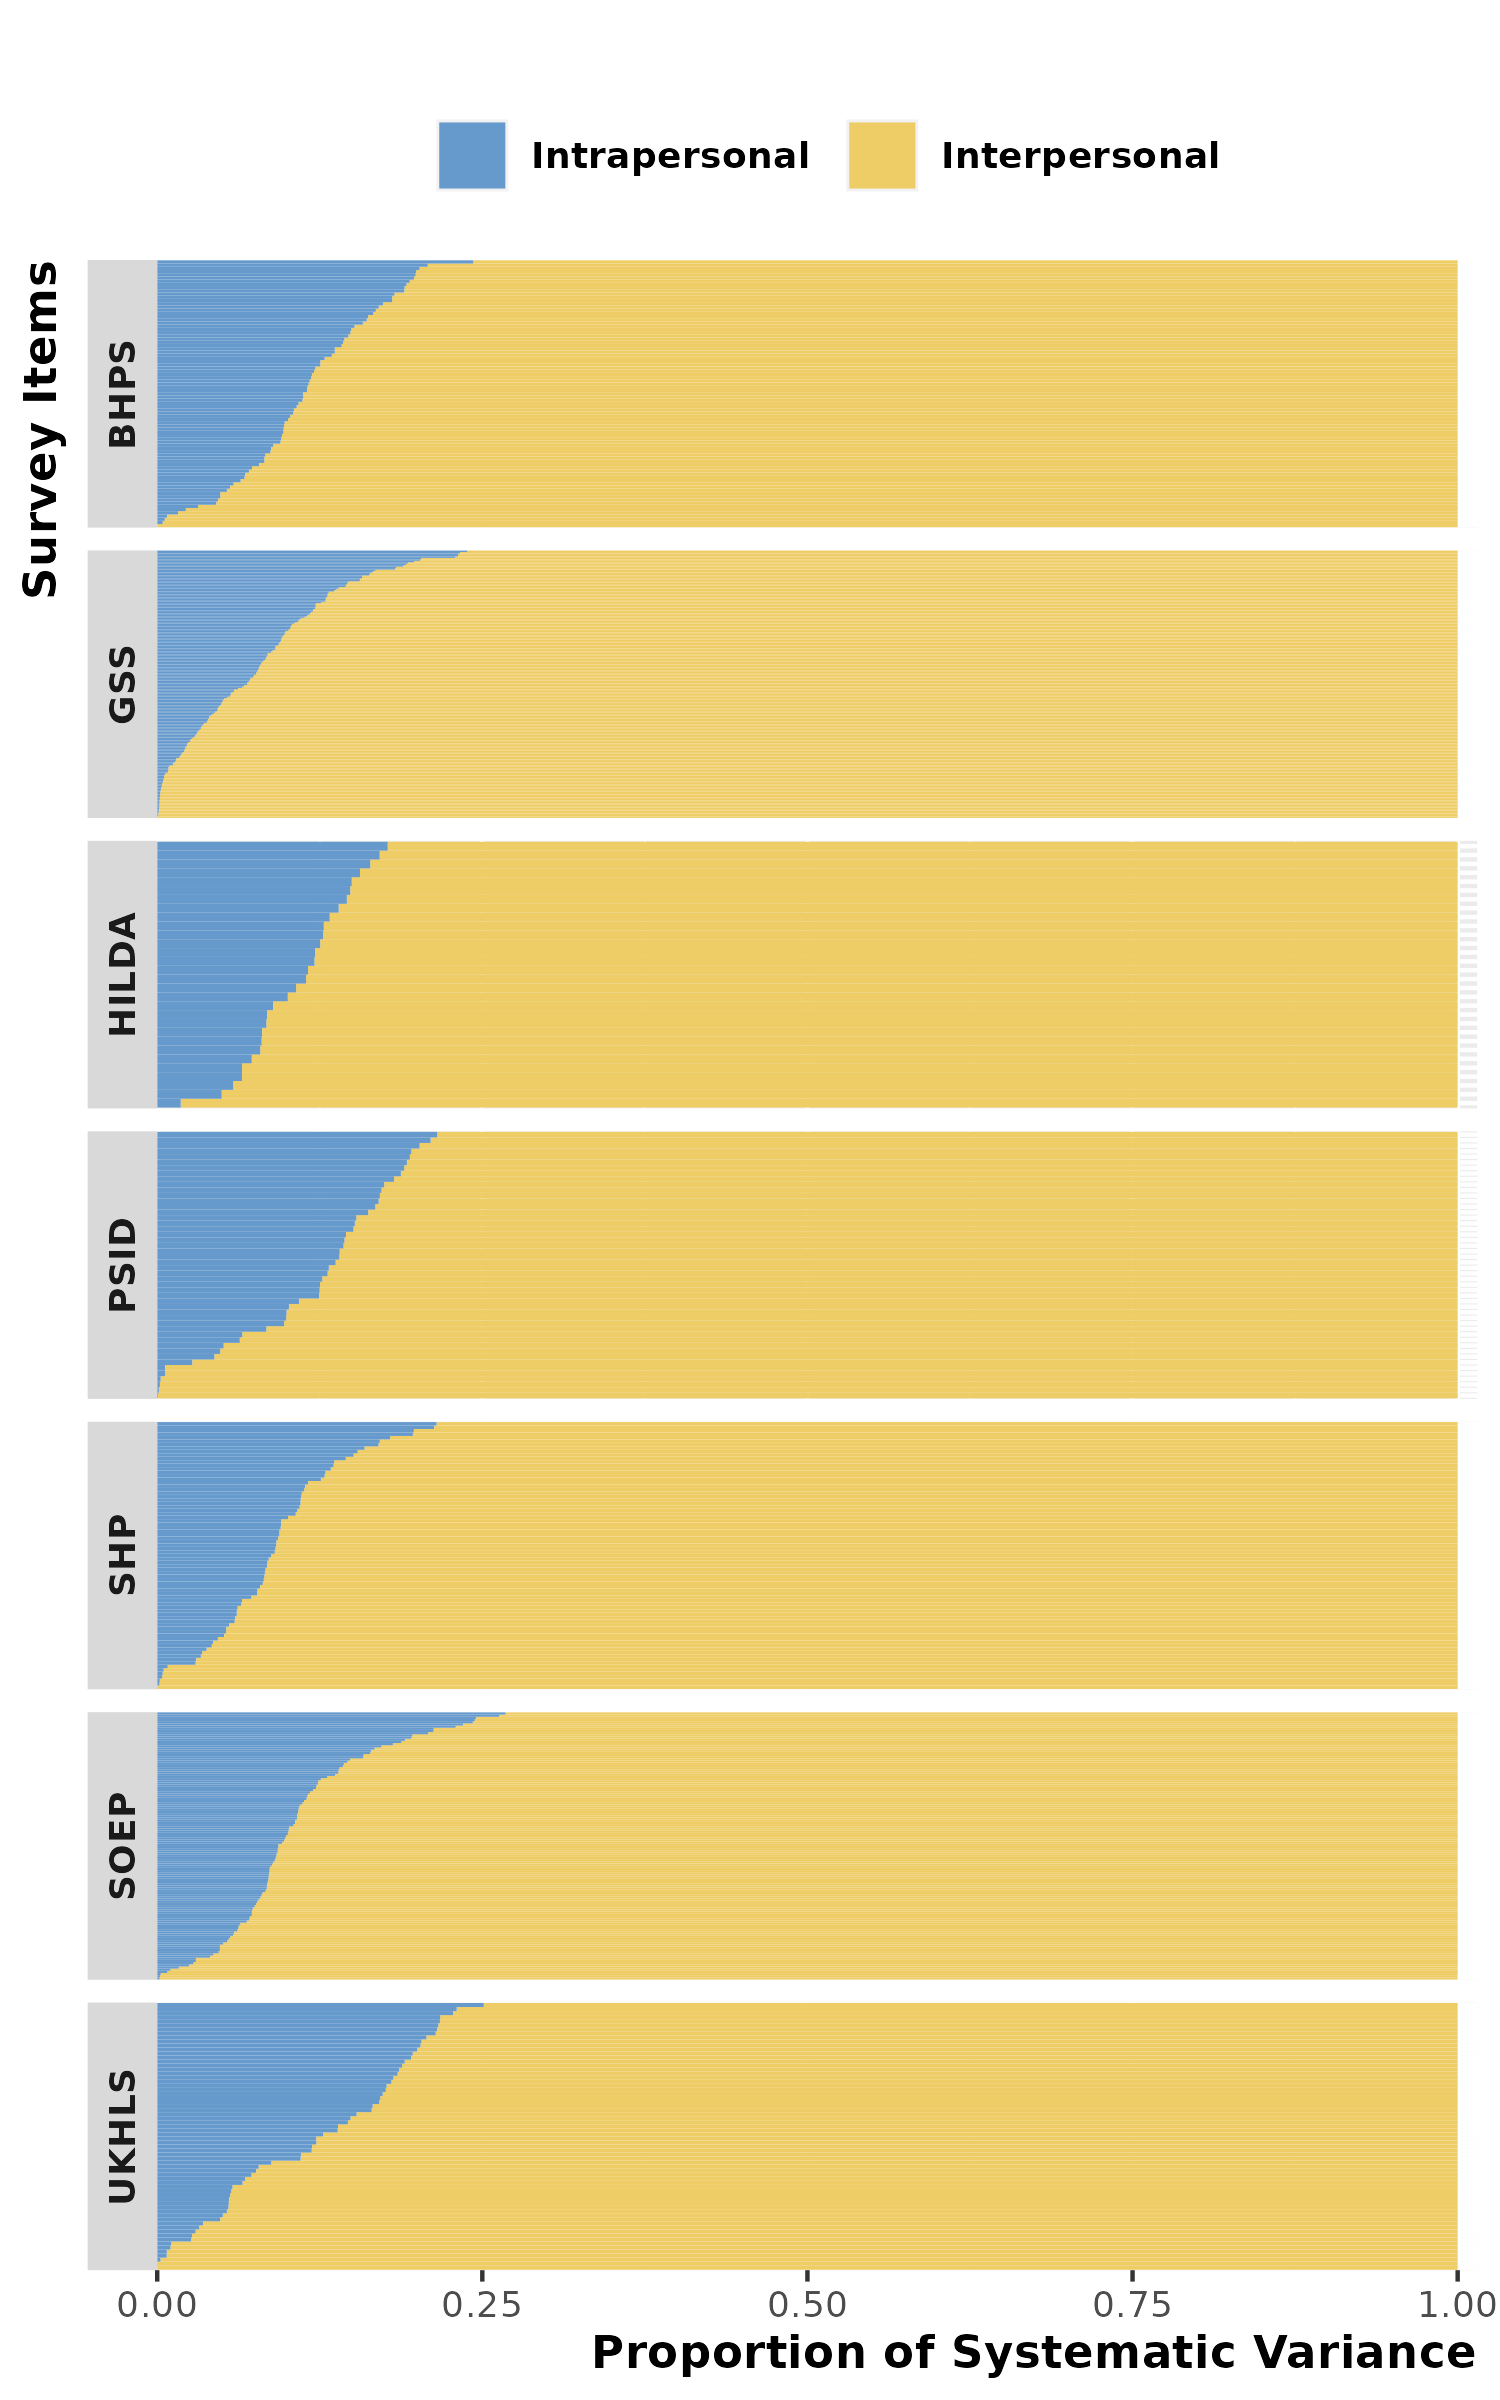
\includegraphics[width=1\linewidth]{../figures/figure_1}

\end{center}
\footnotesize{\textit{Notes:} The figure shows $\omega$ and 1 - $\omega$ as the proportion of systematic variance attributable to intrapersonal change and interpersonal differences. See Supplemental Materials A for the full set of item values.}
\end{figure}

Across all questions, interpersonal differences account for a much
larger share of the systematic variance in responses than intrapersonal
change. Again, this is to be expected. Interpersonal differences capture
not just pre-adult socialization, but all accumulated experiences up to
the start of the panel that might influence personal culture.

To the extent that there are differences across the panels, the PSID has
the highest \(\omega\) values with mean .120 and median .135. While we
cannot disentangle features of the sample from features of the questions
asked to each sample, the specific samples for many PSID questions have
lower average ages than those from other panels. To the extent that
younger respondents might be more likely to make durable changes of
opinion, these higher estimates of intrapersonal change might reflect
the distinct age profile of respondents in this sample. At the other
end, the GSS has the lowest range of \(\omega\) with mean .073 and
median .069. This potentially reflects the fact that the GSS observes
people for a shorter duration, on average, than the other panels. If,
consistent with life course adaption theories, people are more likely to
make significant cultural changes the longer we observe them, then
duration likely affects the range of \(\omega\) (a point we explore more
below). However, the GSS results are still consistent with results from
the other panels.

While there are some differences between panels, these differences are
small compared to the differences within panels. For about 6 percent of
items, \(\omega\) is greater than 0.20. These questions tend to ask
about objectively changing external referents (e.g., confidence in
specific government leaders or political parties), life satisfaction, or
current financial position. At the other end, questions about religious
identification, views on gender roles, and support for civil liberties
tend to have very low estimates of intrapersonal change.

In contrast to the tournament of models approach, quantifying change
this way allows us to explore variation in the relative importance of
intrapersonal change across questions that all show evidence of change.
For example, Kiley and Vaisey (2020) found that confidence in the press
and confidence in religious leaders were both characterized by active
updating. Our results show that intrapersonal change is much more
important for explaining variance in confidence in the press (0.164)
than confidence in religion (0.049), even though both are updating.

Appendix A shows the distribution of \(V(D)\) and \(V(C)\) across
panels, and Supplemental Materials A presents the estimated proportion
of variance attributable to interpersonal differences and intrapersonal
change, the estimated values of \(\omega\), and the proportion of
residual variance for each question. Interpersonal differences are
almost always the largest component of the total variance and tend to
account for between 55 and 70 percent of total variance, while
intrapersonal change is always the smallest, typically accounting for
between 3 and 8 percent of total variance. Residual variance tends to
account for between 22 and 37 percent of variance, though on several
questions residual variance is greater than 50 percent. This might
indicate survey items with low reliability or ones that capture
genuinely rapid fluctuations.

As we noted above, the substantive importance of a given amount of
intrapersonal change depends on a range of factors, including how long
the panel runs, whether assumptions about linear change hold, and
whether the panel is capturing a distinctly turbulent period or a
distinctly stable period for the relevant item. However, if we assume
that the period under observation is ``typical'' for a question---not a
time of extremely heightened (or lowered) sensitivity or change---then
it does not seem realistic that intrapersonal change accounts for a
large share of the cultural differences we see in the world.

\hypertarget{meta-analysis}{%
\subsection{Meta-Analysis}\label{meta-analysis}}

Figure 2 plots the results from a linear regression of \(\omega\) as a
function of question, panel, and sample features. These models also
include fixed effects for panels and topics, so coefficients reflect the
association within a panel and topical domain.

\begin{figure}[htp]
\begin{center}
\caption{Regression Model Estimating $\omega$}

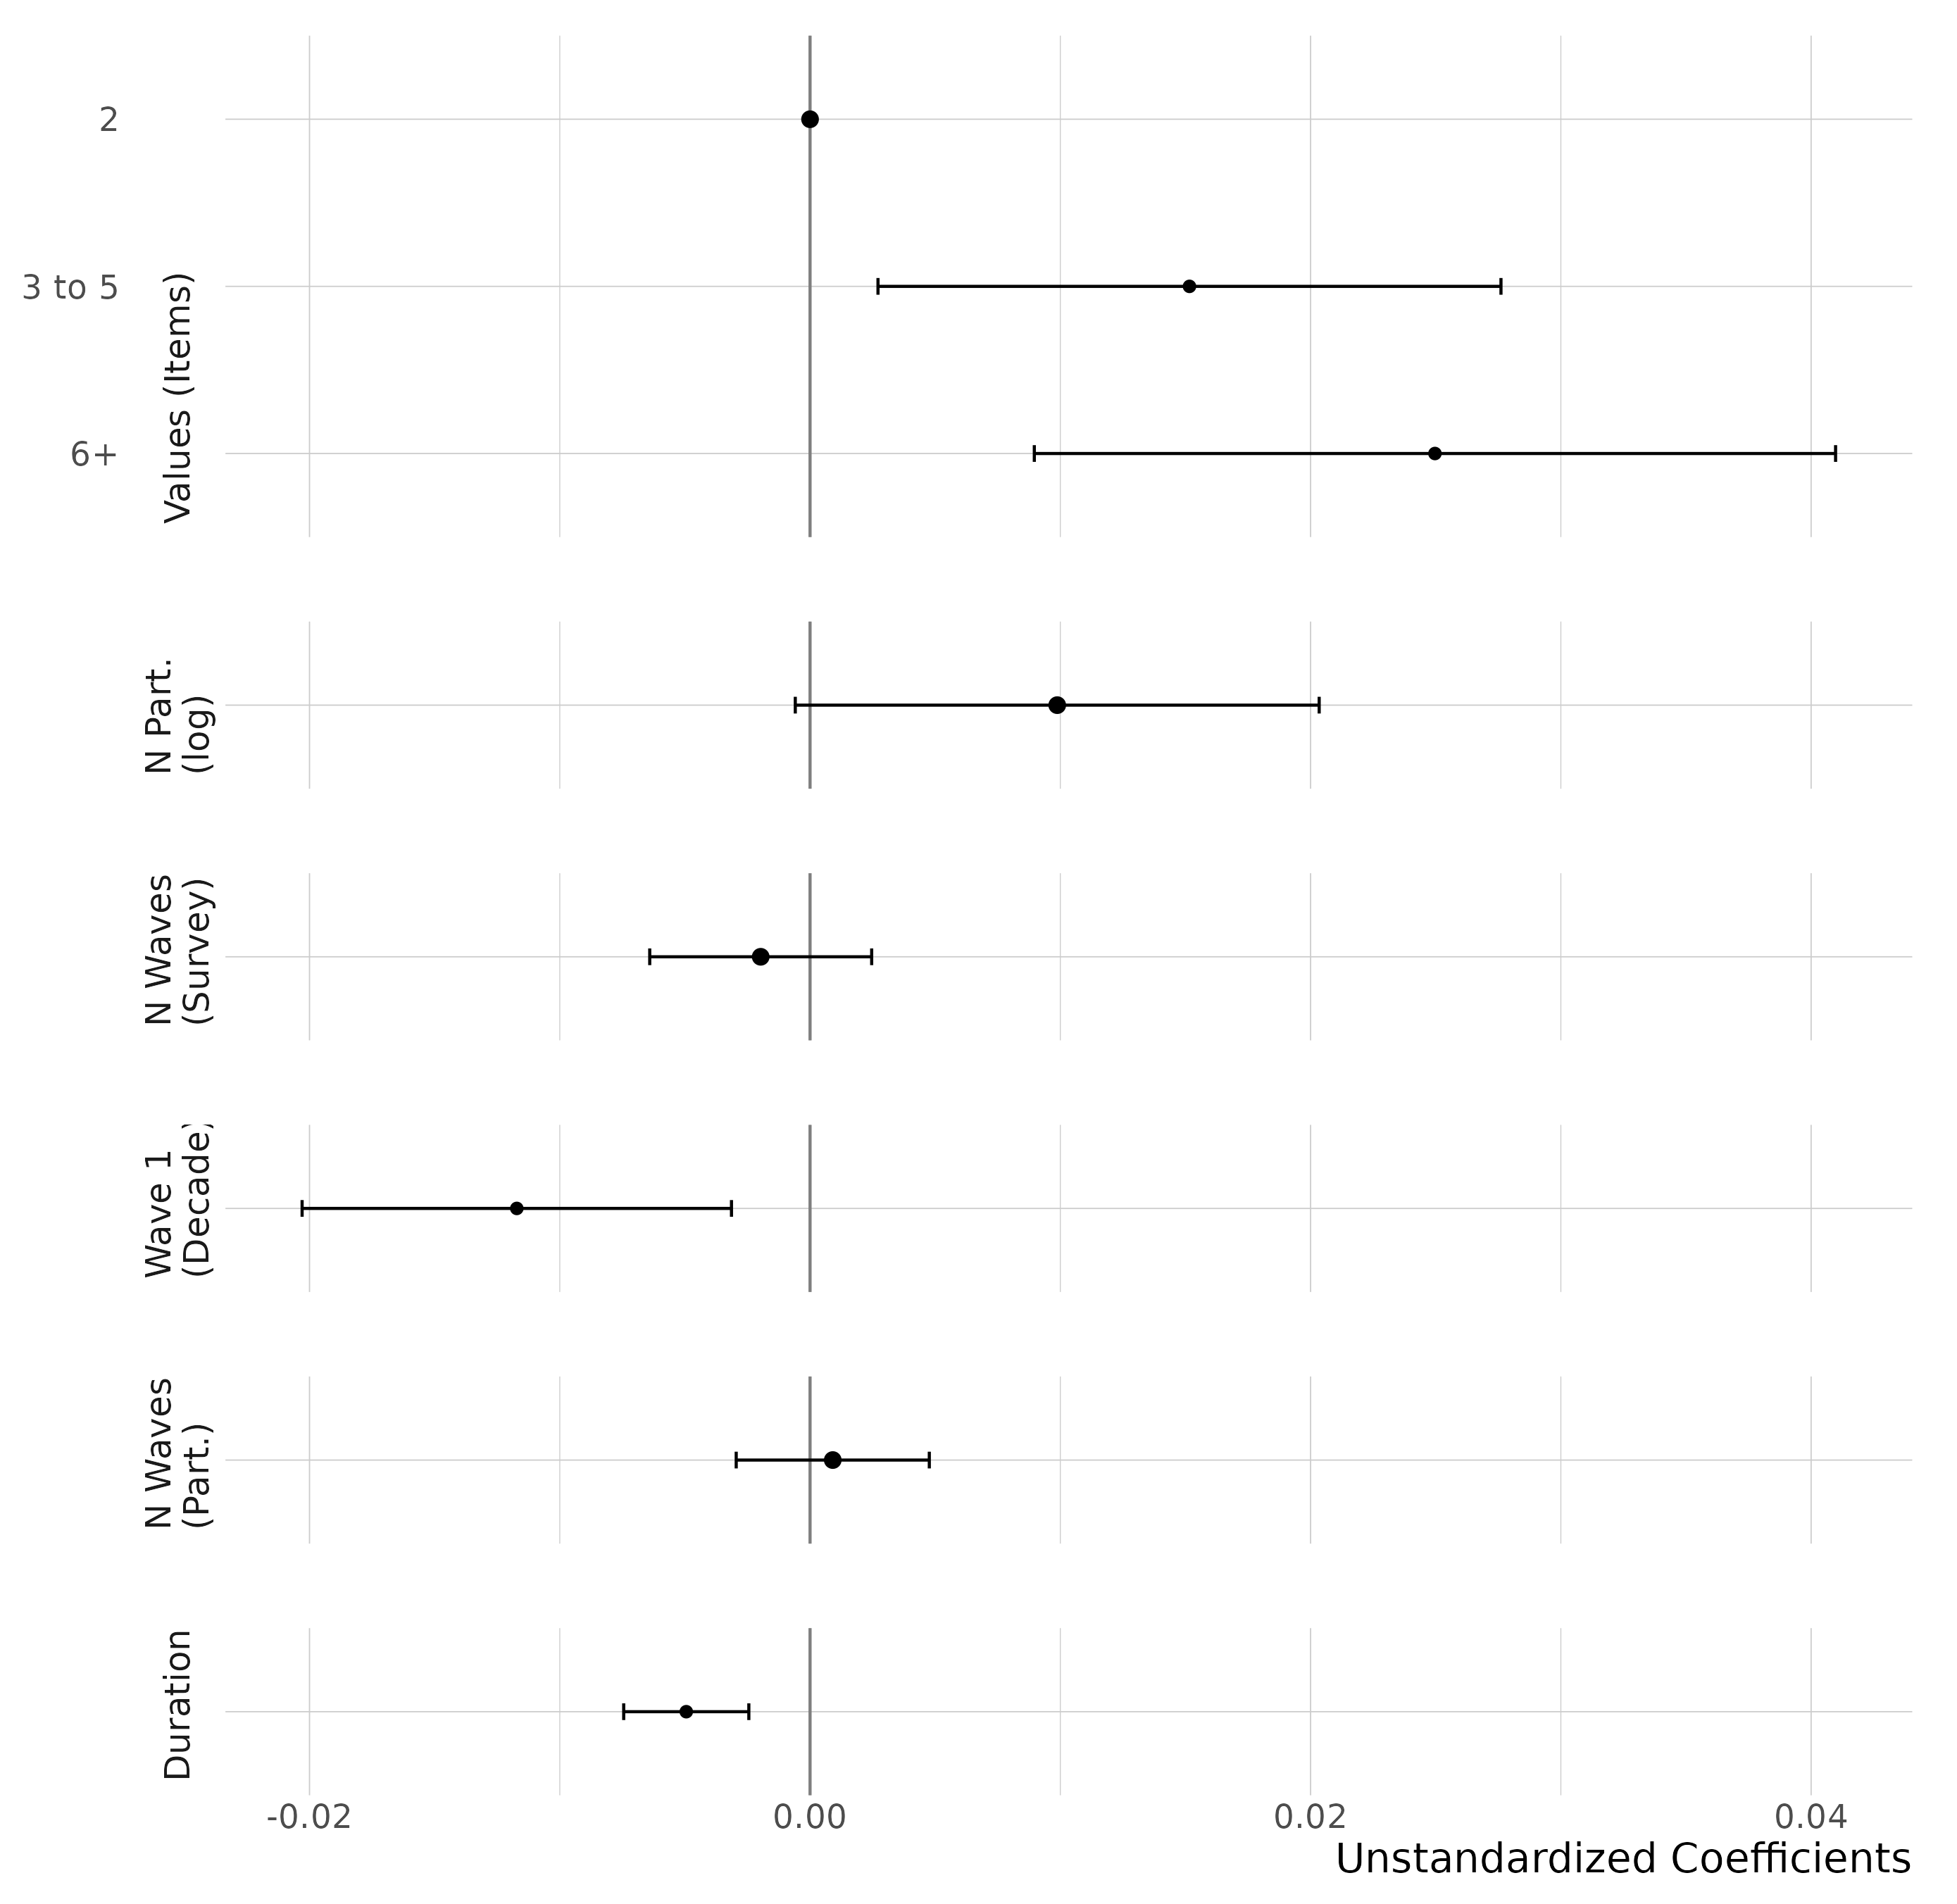
\includegraphics[width=350px]{../figures/figure_2}

\end{center}
\footnotesize{\textit{Notes:} The model estimates the proportion of systematic variance attributable to intrapersonal change. It includes the log of the number of participants, the number of waves the variable was asked (capped at t = 10 for each item), the date of the first wave (measured as the year minus 1968 divided by 10), number of waves the question was asked averaged across participants, duration in years per item averaged across participants, and panel and topic fixed effects. Coefficients are estimated from suppressed intercept model based on predictions at participants' wave mid-point. Survey indicators and item topics not shown. See Supplemental Materials B for the full set of coefficients.}
\end{figure}

Figure 2 shows that the more response options respondents are given and
the larger the sample, the larger the values of \(\omega\). We interpret
these coefficients as suggesting greater resolution on a question makes
it easier to detect and model change. The earlier a question was asked,
even net of how long it was been asked, the lower \(\omega\).

Although we did not state expectations for how question content would
relate to \(\omega\), some of the associations between question
structure, panel duration, and panels themselves might be driven by
differences in the topics addressed by each panel. To address this, we
followed Hout et al. (2016) and Lersch (2023) in coding each question as
falling into one of nine different topical domains and included these as
indicator variables in the meta analysis. Supplemental Materials B
presents the estimates for these topic indicators. They show some
associations with \(\omega\), with questions about subjective SES;
social life, social cohesion, and trust; environment and climate; and
health and morale showing larger \(\omega\) values than questions about
religion and spirituality; politics, government and the economy; and
gender and family.

The most notable result in the meta analysis is the negative coefficient
attached to the duration of years covered by the question on average
across participants. The longer a question is observed, the less is the
value of \(\omega\). Theories of personal cultural change that link
changes in personal culture to social experiences, including the LCAM,
suggest that the longer we observe respondents, the more likely people
are to undergo potentially transformative experiences and therefore the
more variance would be attributable to intrapersonal change. Finding a
negative coefficient here seems to challenge that assumption.

As a further test of this finding, we compared the \(\omega\) values
when using the full duration of a panel compared to when we dropped the
final wave for each participant and therefore reduced the total duration
of observation for the question. If the coefficient reflects a true
negative effect of duration on \(\omega\), we should see that same
effect within questions. Results from this analysis are presented in
Appendix B and contradict the coefficient from the regression model;
with a few exceptions, we found that the longer we observe the same
question, the higher \(\omega\) is. We interpret this combination of
findings as suggesting that the kinds of questions asked for a longer
time period tend to demonstrate less intrapersonal change than questions
asked over shorter periods, rather than a true function of time. This
supports the conclusion that the GSS shows less intrapersonal change
because of its shorter duration.

\hypertarget{college-and-change-in-political-culture}{%
\subsection{College and Change in Political
Culture}\label{college-and-change-in-political-culture}}

These results mostly re-frame and align previous findings, but the value
of our approach lies in its ability to extend the debate to a broader
set of theoretical questions. To show this potential, we turn to a
specific empirical example: the relative importance of intrapersonal
change and interpersonal difference for explaining cultural variation by
level of education.

Previous work has established a positive relationship between education
and attitude stability, especially on issues related to American
politics. This stability is often attributed to education facilitating
``chronic information'' -- a general understanding of and attention to
the domain of American politics, including the positions held by major
parties and political figures and how issues relate to one another at a
logical or socio-logical level (Alvarez and Brehm 2002; Boutyline and
Vaisey 2017; Zaller 1992). These perspectives argue that because college
graduates have more knowledge of American politics, they are better able
to consistently connect the considerations in their cognition with the
answer choices they are presented with in a survey.

This work has tended to focus on the fact that college-educated
Americans give responses that are less likely to be affected by
measurement error or short-term influences than the rest of the
population (Alwin 2007; Zaller 1992). But this focus on the
non-systematic or residual component of variance across groups lumps the
two systematic forms of difference together. That is, it obscures the
fact that the amount of interpersonal differences and intrapersonal
change might also differ across these groups.

There are theoretical reasons to believe that education might be
associated with either more or less intrapersonal change. On one hand,
because college graduates are more connected to mainstream discourse and
elite signals, they might be more likely to make durable changes in
response to the emergence of new information, new issues, or political
realignments, while those without chronic information might display more
variance around an unchanging baseline (Zaller 1992). Conversely, it
could be that the observed stability of the college educated reflects
the fact that they have already formed durable opinions and are
relatively closed off to new information. If this is true, college could
be understood as a formative experience that solidifies some dimensions
of personal culture. Perhaps for those who do not attend college, later
life experiences might prove more important in forming or changing
personal culture, as these experiences potentially provide information
that college-educated peers have already received.

To compare these competing propositions, we calculate \(\omega\) values
separately for people with at least a bachelor's degree and people with
less than a bachelor's degree at wave 1\footnote{A small number of
  respondents report different highest degrees at wave 1, wave 2, and
  wave 3. Some of this is due to measurement error, and some of it is
  due to a small number of people obtaining a higher degree during the
  four years of the panel. Estimating the panel with highest at wave 1
  or highest degree reported across the panel produces functionally
  identical results.} of the three General Social Survey's panels. We
focus on the GSS because it contains the largest number of questions
tapping general political dispositions, which is the domain where
education has proven particularly relevant for understanding attitude
stability. The GSS also covers a turbulent window of American politics
from 2006 to 2014. This window covers the start of the Great Recession,
debates about federal intervention in and regulation of Wall Street, the
election of Barack Obama as the first black U.S. president, debates
about the role of the federal government in the health care sector, the
emergence of the Tea Party, and political realignment and clarification
on the issue of gay marriage, among other topics.

Figure 3 plots the distribution of differences in \(\omega\) values
between people with at least a bachelor's degree and people with less
than a bachelor's degree at wave 1 of the panel for 183 GSS items.
Values greater than 0 indicate that intrapersonal change accounts for
more systematic variance among college graduates than among those
without a college degree, while values less than 0 indicate the
opposite.

\begin{figure}[hbt]
\begin{center}
\caption{Difference in $\omega$ Across College Graduates and Non-Graduates}

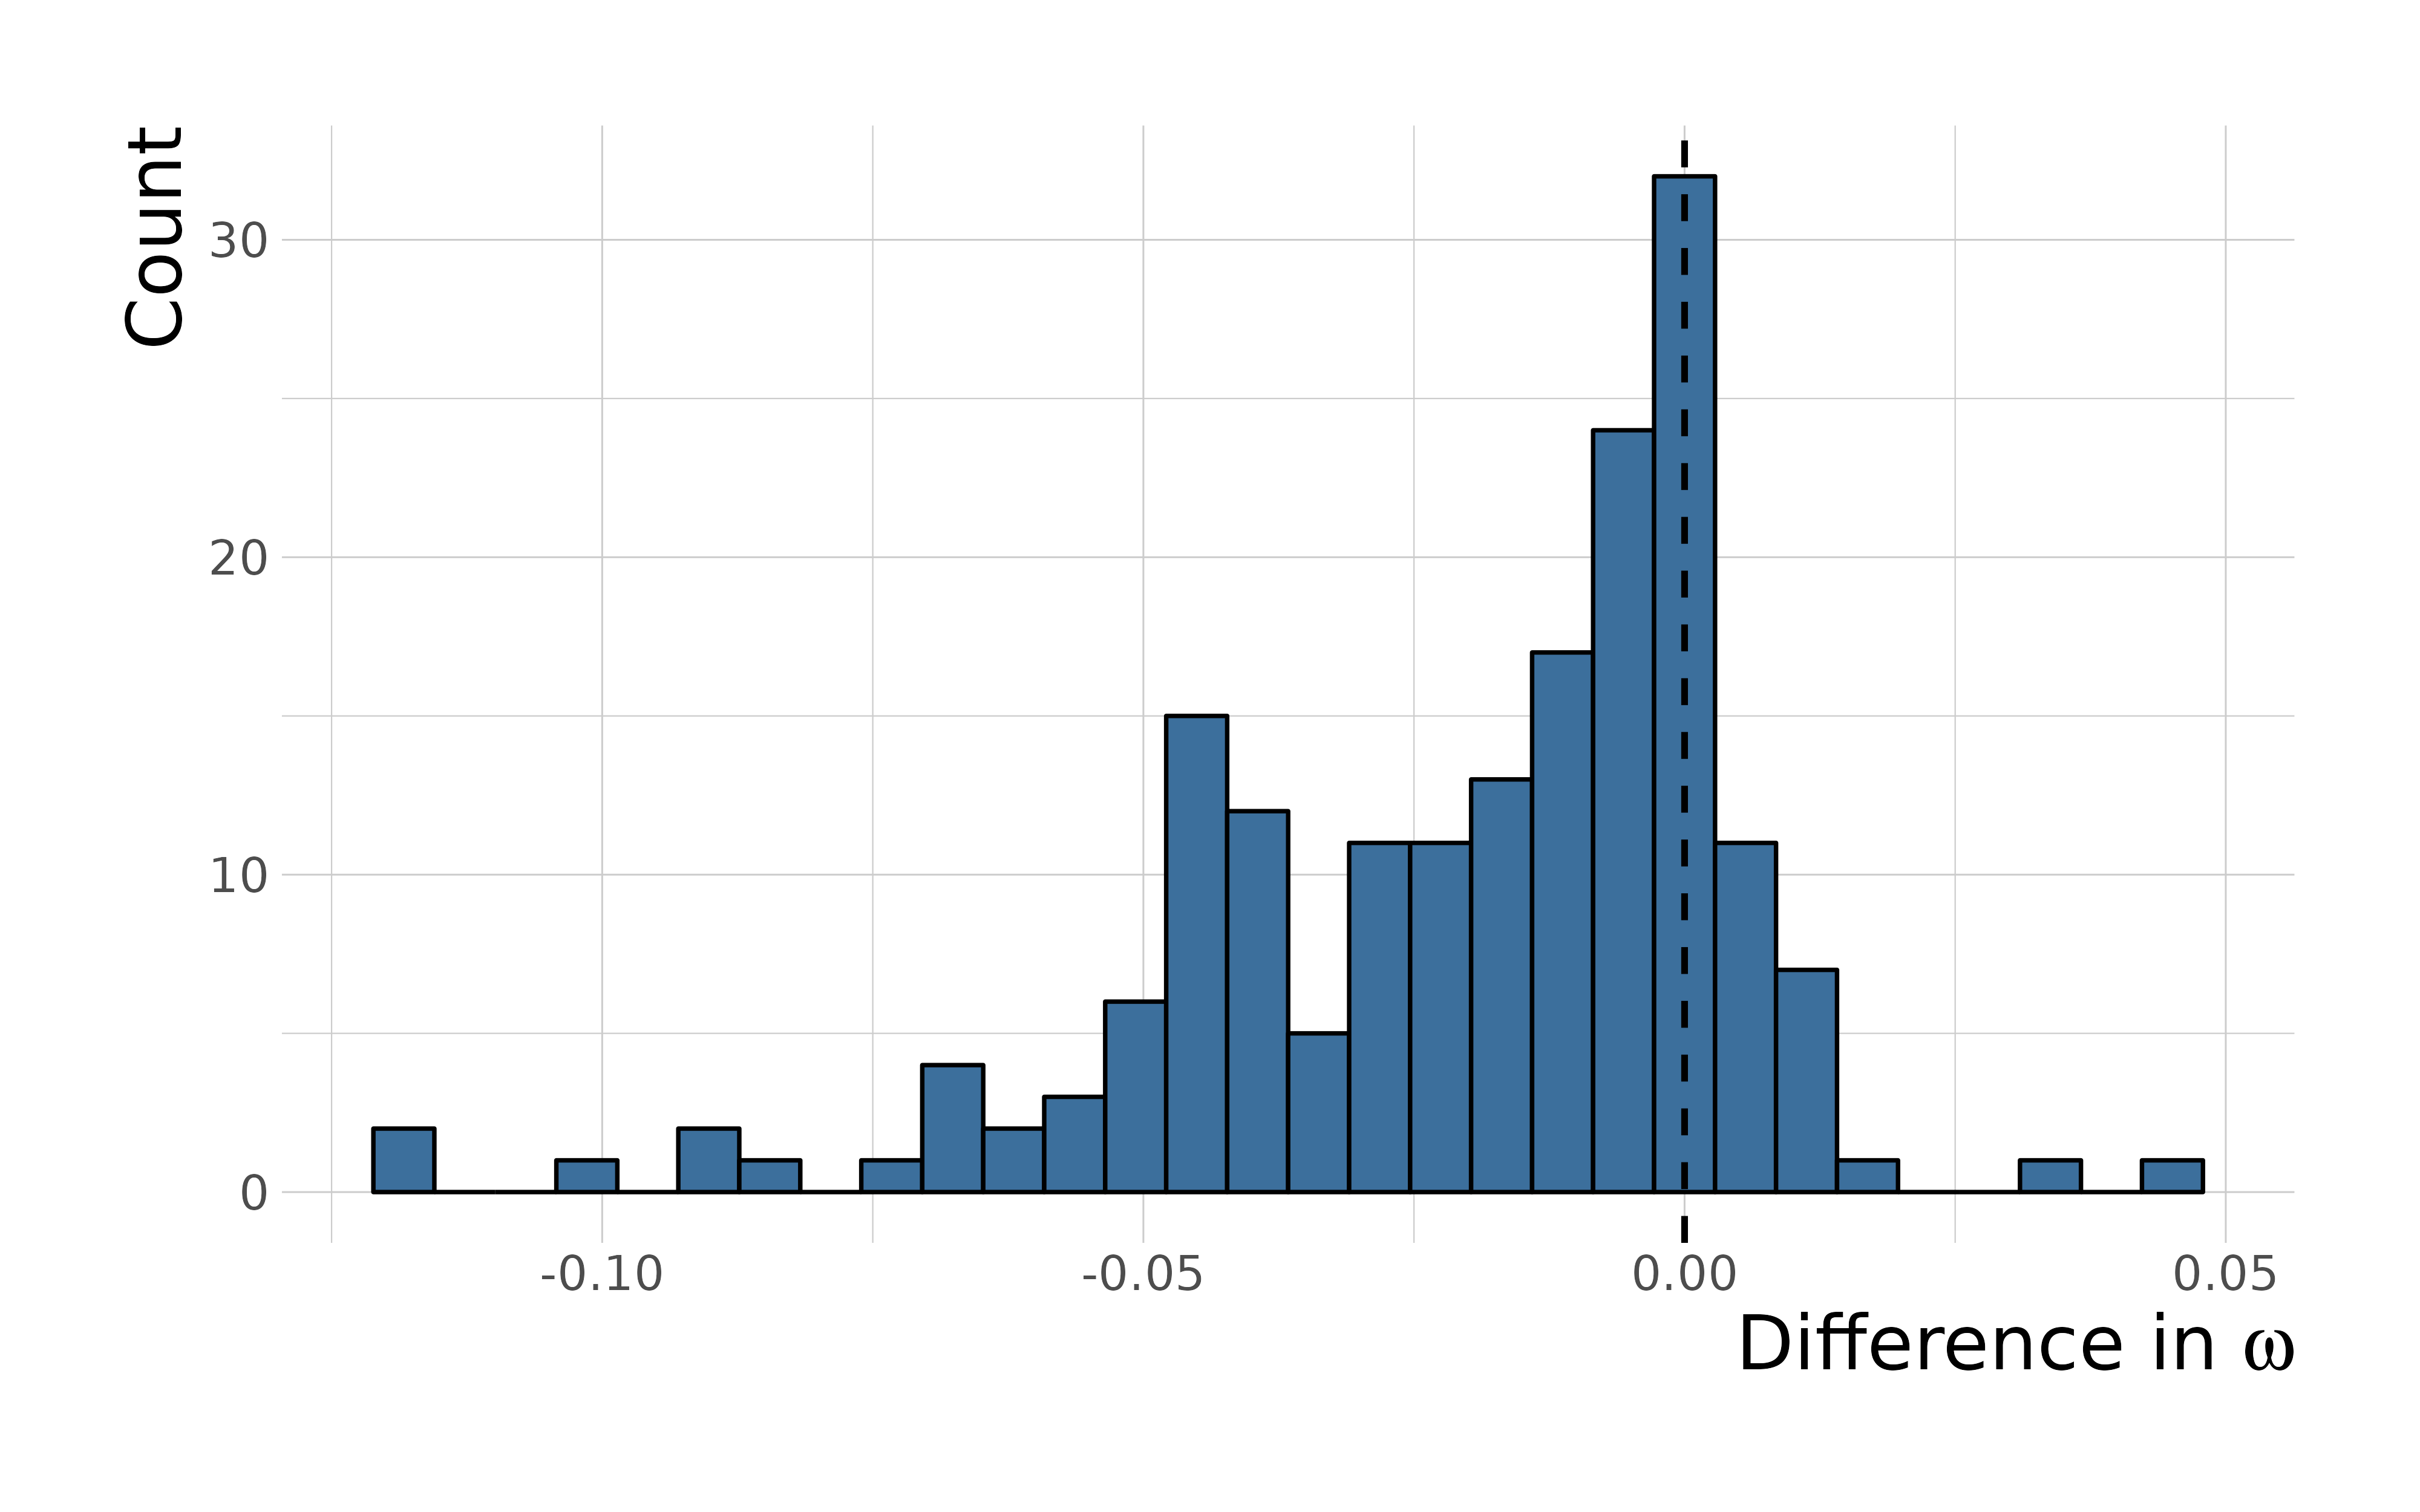
\includegraphics[width=450px]{../figures/figure_3}

\end{center}
\footnotesize{\textit{Notes:} The figure shows the difference in $\omega$ values across college graduates and college non-graduates. Values above (below) 0 means that those with college degree have higher (lower) variance of intrapersonal change. The dashed red line marks 0 difference.}
\end{figure}

There is a clear pattern in Figure 3: for more than 80 percent of these
GSS items, intrapersonal change is a larger component of systematic
variance for people without a college degree. While most of these
differences are small in absolute terms (less than 2 percentage points),
several are greater than 5 percentage points. Given the distribution
observed in Figure 1 showing that the systematic variance attributable
to intrapersonal change averages around 0.09, a 5 percentage point
difference between groups is quite substantial.

To more clearly illustrate some of these differences, we highlight eight
questions designed to tap general political dispositions: partisan
identification (Democrat vs.~Republican) and ideological identification
(liberal vs.~conservative) on seven-point scales; four questions about
the government's role in improving the condition of the poor, paying
people's medical bills, giving special treatment to black people, and
doing things that private businesses could do, measured on five-point
scales; a question about whether the government should do more to reduce
income differences, measured on a seven-point scale; and one question
about whether black people should be given preferences in hiring,
measured on a five-point scale. We present estimates of \(\omega\) for
these eight questions, for both education groups, in Figure 4.

\begin{figure}[hbt]
\begin{center}
\caption{Difference in $\omega$ Across College Graduates and Non-Graduates on Political Culture}

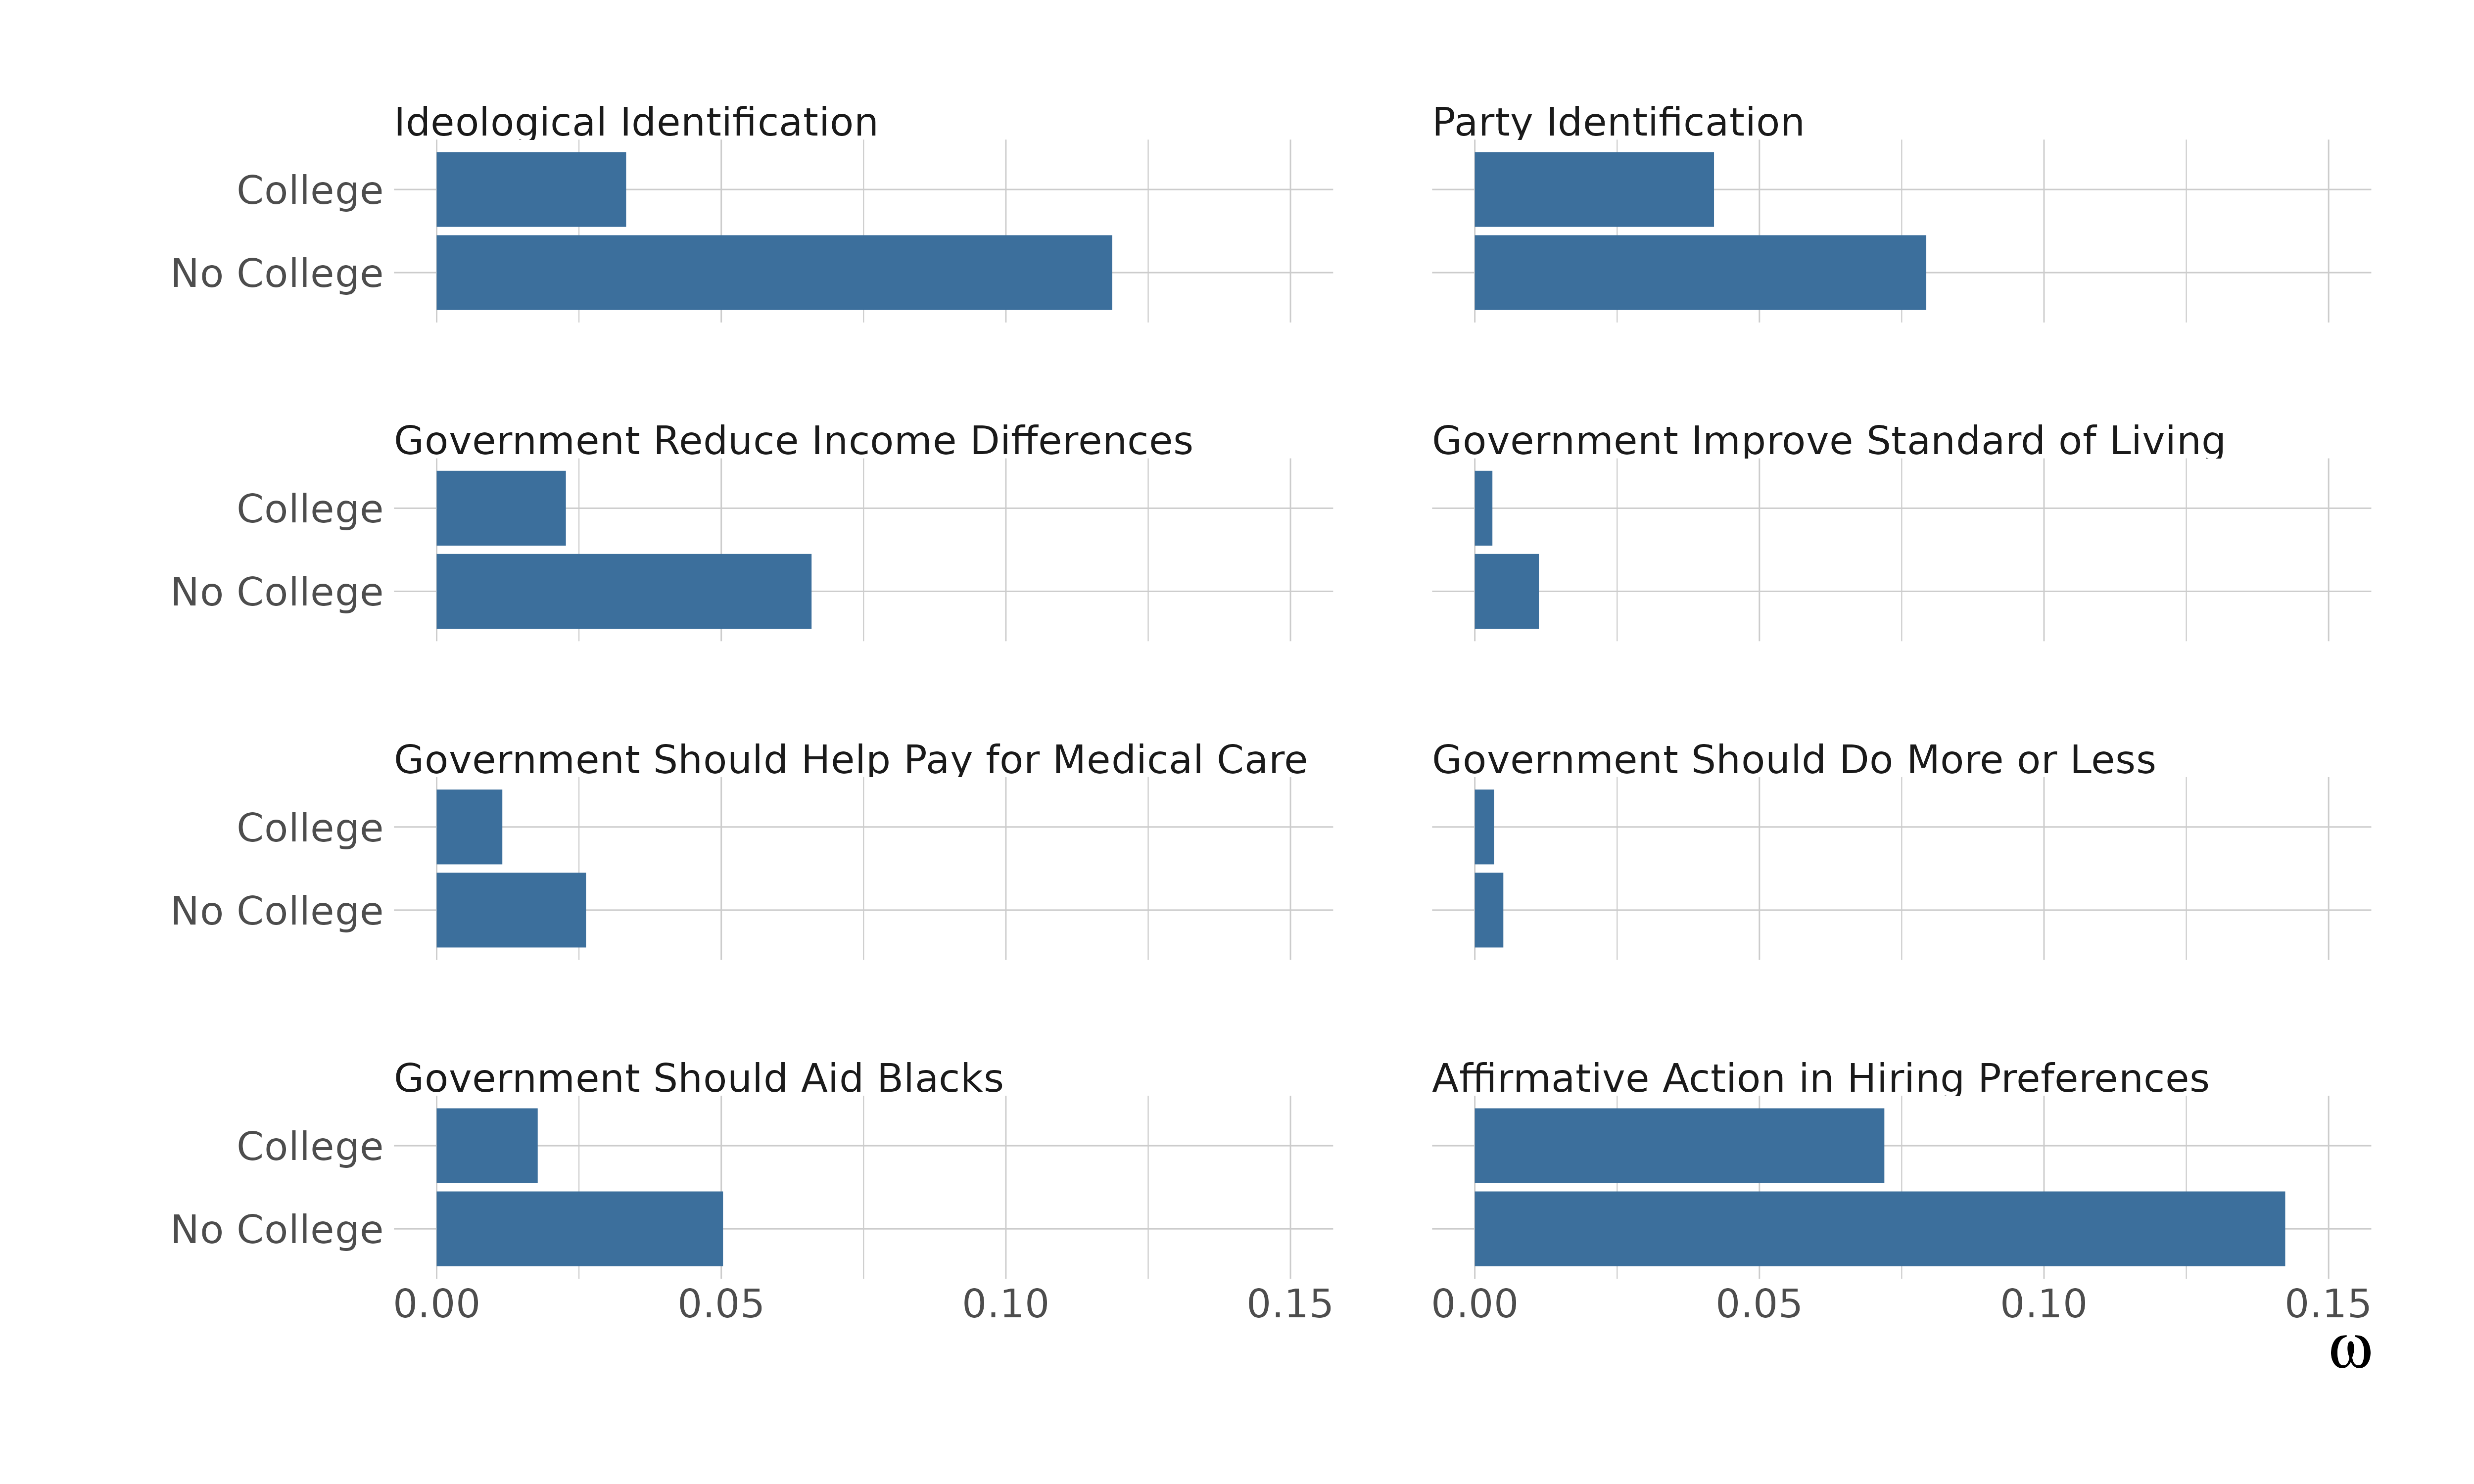
\includegraphics[width=450px]{../figures/figure_4}

\end{center}
\footnotesize{\textit{Notes:} $\omega$ values across college graduates and college non-graduates on 8 political culture items from the General Social Survey (2006-2014).}
\end{figure}

On all eight questions presented in Figure 4, \(\omega\) values are
smaller for people with a college degree, meaning intrapersonal change
is less common among them. There are also large differences in
\(\omega\) values across questions for both groups. For example, on the
question of whether the government should try to solve more problems or
leave those problems to be solved by private businesses (``government do
more or less''), less than 1 percent of the systematic variance is
attributable to intrapersonal change for both groups. In other words,
while people might vacillate on this question at random (37 percent of
variance is residual for this question), there is functionally no
evidence that people make systematic changes of opinion on this issue
during the GSS panel.

In contrast, partisan identification and political ideology both show
larger values of \(\omega\) than most other questions, as well as a
larger absolute difference by degree status. Compared to the other
questions, intrapersonal change plays a much larger role in accounting
for partisan identification and political ideology. And this is
particularly true for respondents who do not have a college degree; the
\(\omega\) value for ideological identification among non-college
educated respondents is almost four times that of college-educated
respondents.

It is worth pointing out that this meaningful difference in \(\omega\)
values across education groups and across questions would not have been
detectable using previous methods. For partisan identification and
political ideology, both college-educated respondents and people with
less than college degree would likely favor the AUM or LCAM over the SDM
because these questions both show evidence of some members of the
population making \emph{some} intrapersonal change. In other words, the
tournament of models obscures the fact that the relative importance of
intrapersonal change differs across these two groups, that intrapersonal
change explains more systematic variance for ideological identification
and partisan identification for people without a college degree, and
that there appears to be more durable change on questions of affirmative
action than on questions of government aid to black Americans.

We believe these patterns shed new light on the mechanisms underlying
differences in attitudes and behavior across groups. Something about
college attendance seems to crystallize personal culture. While these
results should not be interpreted as causal effects of attending college
-- they are potentially confounded by age, social class, race, gender,
and other factors that explain selection into higher education -- they
open up a set of new questions and dynamics to explore.

\hypertarget{discussion-and-conclusion}{%
\section{Discussion and Conclusion}\label{discussion-and-conclusion}}

The objective of this paper is to intervene in the recent debate on
whether people change their personal culture -- their attitudes,
beliefs, values, and practices -- as they move through their adult life.
Instead of falling back on a ``tournament of models'' approach (Lersch
2023: p.~228) to proclaim victory for a particular answer to this
question, our goal is to refocus the debate to the theoretically more
productive question of the relative importance of intrapersonal change
for explaining differences in the personal culture. We propose a new
approach that quantifies the amount of observed systematic variance that
is attributable to either interpersonal differences at baseline or
intrapersonal change over the duration of a panel.

Applying our proposed measure, \(\omega\), to 609 survey items from all
of the panel datasets previously discussed in this debate revealed a
consistent pattern. Nearly all questions show evidence of people making
some durable, intrapersonal change over time. Some show notably high
amounts of intrapersonal change. For some questions about life
satisfaction or views on government benefits, it seems plausible that
differences in adult experiences predominantly account for observed
differences between people.

However, intrapersonal change is often substantially less pronounced
than interpersonal differences, accounting for less than 10 percent of
systematic variance on average across all datasets. On numerous
questions, like those on civil liberties, abortion, generalized trust,
and civic duty, the systematic variance attributable to intrapersonal
change is essentially zero. For these questions, it seems there is not
enough cultural change during adulthood to warrant attributing the
differences we observe to experiences and social transitions; instead,
the primary source of the observed differences appears to stem from
experiences in childhood, adolescence, and early adulthood.

More than adjudicating past positions in this debate, the approach we
presented in this paper will enable scholars to explore more precisely
the relative contributions of change and stability in explaining
variation in personal culture, as well as how these contributions might
differ across populations. To illustrate this, we showed how the amount
of cultural difference explained by intrapersonal change varies
substantially by survey item but also by individuals' characteristics
such as their education. While age and other factors related to college
completion might confound this pattern, it suggests that college
completion may crystallize personal culture to an extent that renders
later adult experiences on political dispositions less influential.

\hypertarget{limitations}{%
\subsection{Limitations}\label{limitations}}

Although we believe it is a major advance on previous work, the approach
we outline here has important limitations. We allocate all systematic
variance to one of two sets of theoretical processes: intrapersonal
change and interpersonal differences at baseline. Our approach does not
quantify the proportion of people who ``change,'' nor can we be sure
that the amount of interpersonal change we detect is driven by many
people making small changes or a few people making large changes.

Our results and interpretations also hinge on how we have defined
change. As does the LCAM, our approach treats cultural trajectories as
varying linear slopes for each respondent, thus assuming that change is
a linear function of time. This assumption simplifies reality in which
change likely also takes non-linear and discontinuous forms. People
might jump from one ``stable'' disposition to another or experience a
``turning point'' in their lives that upsets an otherwise stable
trajectory. In parts, our assumption of linearity is a limitation of the
data, as most questions are only observed for three to six waves. Panels
with more waves might allow researchers to loosen this assumption to
test alternative, more flexible models of change.

Similarly, our approach assumes that durable change is unidirectional.
This is a sensible assumption on short panels where classifying change
that lasts less than two years as durable seems unreasonable.
Practically, it means that the variance produced by people making
durable changes in their cultural dispositions to then return to a
previous state later in life is classified as residual variance, rather
than intrapersonal change. Longer panels and more flexible definitions
of ``change'' might allow us to account for such trajectories.

Finally, we had chosen to examine the broadest array of measures of
personal culture available to us, ranging from religious beliefs and
core values, to policy preferences, and even to the importance of
different features when buying a new car across five countries
(Australia, Germany, Switzerland, the United Kingdom and the United
States). Nevertheless, our findings remain limited to the kinds of
questions that are asked in panel surveys and in the contexts they were
administered, reflecting issues of general (national) politics, gender
roles, immigration and race relations, and general well being. Although
we have no reason to believe results to be different, our findings do
not directly speak to other dimensions of culture such as artistic
tastes, leisure activities, and time use.

\hypertarget{implications-for-cultural-sociology}{%
\subsection{Implications for Cultural
Sociology}\label{implications-for-cultural-sociology}}

Despite these limitations, we believe our method and findings have
important implications for social science research. Sociologists
interested in understanding cultural differences have largely asked
about the \emph{existence} of cultural change in adults (e.g., Kiley and
Vaisey 2020; Lersch 2023; Vaisey and Kiley 2021). Yet this approach has
inadvertently limited the debate. In any population, \emph{some} degree
of adult cultural change is inevitable. Although ideal types like the
settled dispositions and active updating models are useful, no
theoretical perspective would expect either early life socialization or
adult intrapersonal change to be the sole source of one's personal
culture. Our results reinforce this point, showing the relevance of both
factors and allowing their precise quantification.

This and other recent findings (Quinn et al. 2023; Stewart and Berkman
2023) suggest that it is theoretically more productive to measure the
relative importance of these two components in concrete, substantive
cases. Drawing a unified conclusion from survey items measuring various
cultural forms on different scales and across different time frames is
challenging. Nevertheless, the general pattern suggests that, for most
items, intrapersonal change in adulthood is not the primary reason for
the differences we see between people in the world.

We are not claiming that adults remain static or that their changes are
inconsequential. Even quantitatively minor shifts, such as a 2
percentage-point change in support for gay marriage, can have massive
ramifications. While the majority may remain consistent in their views,
understanding the underlying mechanisms of even such numerically minor
shifts remains a crucial task for the sociology of culture.

Our findings suggest that understanding variation in personal culture
requires examining the conditions and experiences of early life. While
sociological research often focuses on transitions between social roles,
changes in social networks, or the experience of organizational
environments, these factors seem to account for a smaller proportion of
adult differences than early-life experience. Simply put, we need more
work on early-life socialization (Guhin, Calarco, and Miller-Idriss
2020).

This conclusion aligns with a range of recent causal inference work
suggesting that selection effects, rather than treatment effects,
predominantly account for personal cultural differences among
individuals in varied social roles and positions (Campbell and Horowitz
2016; Wodtke 2018). While some people clearly change as they transition
into new roles or environments, this change seems to be insufficient in
magnitude and duration to explain what are often pronounced differences
among people in diverse roles. These and our results suggest that when
observing differences in personal culture across social roles, such as
parenthood, education, or professional authority (Longest, Hitlin, and
Vaisey 2013), or across occupations (Weeden and Grusky 2005), selection
likely plays a large role in explaining these difference, though
exceptions always exist.

Our analysis does not provide an answer as to why intrapersonal change
seems to have limited impact on understanding cultural differences among
adults. The situations that promote durable change in personal culture
might simply be rare during adulthood. Alternatively, it is possible
that adults do encounter opportunities, necessities, and incentives for
change, but their ability or willingness to change decreases. All the
more it is important to research when and how social situations can
provoke durable change in adults.

Related to this, our results regarding education and political views
suggest that the importance of processes that lead to such change can
vary by group. Aligning with life course theories, it seems the
significance of experiences for cultural change may be contingent on
other, prior experiences. For example, factors that shape cultural
dispositions may likely differ for college and non-college graduates;
the latter might be more profoundly influenced by mid-life experiences
than the former in this regard. In trying to understand differences in
personal culture, sociologists should therefore pay more attention to
the heterogeneous effects that various factors including social events,
encounters, and situations can have.

Our findings also have implications for understanding cultural change at
the aggregate level. Given that intrapersonal change accounts for a
relatively small amount of variance among adults, many forms of cultural
change at the aggregate level are necessarily more likely driven cohort
replacement than by contemporaneous social conditions (Underwoood et al.
2022; Vaisey and Lizardo 2016). This likely holds true for cultural
change at the macro societal level as well as the micro level such as
within organizations, political parties, and professions. Our findings
also indicate that the impact of formative experiences, as opposed to
contemporaneous social factors, on cultural change is contingent upon an
individuals' level of education. The weight of these two factors might
thus change as the prominence of education shifts in the life course. If
scholars find similar differences across other social categorizations
like class or race, it might necessitate a more thorough integration of
demographic processes into the analysis of cultural change at the
population level.

\hypertarget{implications-for-survey-research}{%
\subsection{Implications for Survey
Research}\label{implications-for-survey-research}}

Our findings underscore the value of extended panel surveys to advance
theories of culture. On average, non-systematic fluctuations in
responses account for more than four times as much variance as
intrapersonal change, measured as linear change. Differentiating between
the two is therefore crucial for understanding cultural differences and
cannot be done with cross-sectional data. Instead we should extend
panels beyond two waves to gain more leverage to understand when and in
what form personal culture changes.

A key insight from our meta-analysis is that an increase in response
resolution (the range of response options survey respondents are given)
correlates with an increased share of systematic variance explained by
intrapersonal change. This may reflect specific issues being assessed by
survey items using different scales. Alternatively, it might imply that
when intrapersonal changes occurs, they are often subtle with answers
moving from ``agree'' to ``strongly agree,'' rather than from ``strongly
agree'' to ``strongly disagree.'' Such subtle changes require finer
response options to be detected.

Perhaps most important, we need more panel studies on youth. It is very
likely that the majority of adult differences in personal culture are
rooted in different experiences before age 18. By empirically
constraining our analyses to adult experiences, social scientists may
inadvertently concentrate on topics and questions that, while important,
might not be able to help explain major cultural differences in adult
populations.

\hypertarget{conclusion}{%
\subsection{Conclusion}\label{conclusion}}

We believe the approach we outlined here can push past the ``needless
dichotomy'' implicit in the question of whether people change or not
(Lersch 2023). Characterizing questions as displaying change or not can
only take researchers so far, but the question of whether some questions
demonstrate more change than others, or whether some groups are
characterized by more stability than others, has the potential to weigh
in on a broader range of theoretical debates. We hope researchers find
our approach useful as they investigate these questions.

\theendnotes

\hypertarget{references}{%
\section{References}\label{references}}

\hypertarget{refs}{}
\begin{CSLReferences}{1}{0}
\leavevmode\vadjust pre{\hypertarget{ref-alvarez2002}{}}%
Alvarez, R. Michael, and John Brehm. 2002. \emph{Hard Choices, Easy
Answers: Values, Information, and {American} Public Opinion}. Princeton,
N.J: Princeton University Press.

\leavevmode\vadjust pre{\hypertarget{ref-alwin2007}{}}%
Alwin, Duane F. 2007. \emph{Margins of {Error}: {A} {Study} of
{Reliability} in {Survey} {Measurement}}. Hoboken, N.J.: John Wiley \&
Sons.

\leavevmode\vadjust pre{\hypertarget{ref-alwin1991}{}}%
Alwin, Duane F., and Jon A. Krosnick. 1991.
{``\href{https://www.jstor.org/stable/2781642}{Aging, {Cohorts}, and the
{Stability} of {Sociopolitical} {Orientations} {Over} the {Life}
{Span}}.''} \emph{American Journal of Sociology} 97(1):169--95.

\leavevmode\vadjust pre{\hypertarget{ref-bail2018}{}}%
Bail, Christopher A., Lisa P. Argyle, Taylor W. Brown, John P. Bumpus,
Haohan Chen, M. B. Fallin Hunzaker, Jaemin Lee, Marcus Mann, Friedolin
Merhout, and Alexander Volfovsky. 2018. {``Exposure to Opposing Views on
Social Media Can Increase Political Polarization.''} \emph{Proceedings
of the National Academy of Sciences} 115(37):9216--21. doi:
\href{https://doi.org/10.1073/pnas.1804840115}{10.1073/pnas.1804840115}.

\leavevmode\vadjust pre{\hypertarget{ref-bardi2009}{}}%
Bardi, Anat, Julie Anne Lee, Nadi Hofmann-Towfigh, and Geoffrey Soutar.
2009. {``The Structure of Intraindividual Value Change.''} \emph{Journal
of Personality and Social Psychology} 97(5):913--29.

\leavevmode\vadjust pre{\hypertarget{ref-bourdieu1990}{}}%
Bourdieu, Pierre. 1990. \emph{The Logic of Practice}. Stanford, Calif. :
Stanford University Press, 1990.

\leavevmode\vadjust pre{\hypertarget{ref-boutyline2017}{}}%
Boutyline, Andrei, and Stephen Vaisey. 2017. {``Belief {Network}
{Analysis}: {A} {Relational} {Approach} to {Understanding} the
{Structure} of {Attitudes}.''} \emph{American Journal of Sociology}
122(5):1371--1447. doi:
\href{https://doi.org/10.1086/691274}{10.1086/691274}.

\leavevmode\vadjust pre{\hypertarget{ref-brocic2021}{}}%
Broćić, Miloš, and Andrew Miles. 2021. {``College and the {`{Culture}
{War}'}: {Assessing} {Higher} {Education}'s {Influence} on {Moral}
{Attitudes}.''} \emph{American Sociological Review} 00031224211041094.
doi:
\href{https://doi.org/10.1177/00031224211041094}{10.1177/00031224211041094}.

\leavevmode\vadjust pre{\hypertarget{ref-campbell2016}{}}%
Campbell, Colin, and Jonathan Horowitz. 2016. {``Does {College}
{Influence} {Sociopolitical} {Attitudes}?''} \emph{Sociology of
Education} 89(1):40--58. doi:
\href{https://doi.org/10.1177/0038040715617224}{10.1177/0038040715617224}.

\leavevmode\vadjust pre{\hypertarget{ref-christakis2010}{}}%
Christakis, Nicholas, and James Fowler. 2010. \emph{Connected: {The}
{Amazing} {Power} of {Social} {Networks} and {How} {They} {Shape} {Our}
{Lives}}. HarperCollins Publishers.

\leavevmode\vadjust pre{\hypertarget{ref-dellaposta2018}{}}%
DellaPosta, Daniel. 2018. {``Gay {Acquaintanceship} and {Attitudes}
Toward {Homosexuality}: {A} {Conservative} {Test}.''} \emph{Socius}
4:2378023118798959. doi:
\href{https://doi.org/10.1177/2378023118798959}{10.1177/2378023118798959}.

\leavevmode\vadjust pre{\hypertarget{ref-dellaposta2020}{}}%
DellaPosta, Daniel. 2020. {``Pluralistic {Collapse}: {The} {`{Oil}
{Spill}'} {Model} of {Mass} {Opinion} {Polarization}.''} \emph{American
Sociological Review} 85(3):507--36. doi:
\href{https://doi.org/10.1177/0003122420922989}{10.1177/0003122420922989}.

\leavevmode\vadjust pre{\hypertarget{ref-eaton2009}{}}%
Eaton, Asia A., Penny S. Visser, Jon A. Krosnick, and Sowmya Anand.
2009. {``Social {Power} and {Attitude} {Strength} {Over} the {Life}
{Course}.''} \emph{Personality and Social Psychology Bulletin}
35(12):1646--60. doi:
\href{https://doi.org/10.1177/0146167209349114}{10.1177/0146167209349114}.

\leavevmode\vadjust pre{\hypertarget{ref-elder2003}{}}%
Elder, Glen H., Monica Kirkpatrick Johnson, and Robert Crosnoe. 2003.
{``\href{https://doi.org/10.1007/978-0-306-48247-2_1}{The {Emergence}
and {Development} of {Life} {Course} {Theory}}.''} Pp. 3--19 in
\emph{Handbook of the {Life} {Course}}, \emph{Handbooks of {Sociology}
and {Social} {Research}}, edited by J. T. Mortimer and M. J. Shanahan.
Boston, MA: Springer US.

\leavevmode\vadjust pre{\hypertarget{ref-feldman1992}{}}%
Feldman, Stanley, and John Zaller. 1992. {``The {Political} {Culture} of
{Ambivalence}: {Ideological} {Responses} to the {Welfare} {State}.''}
\emph{American Journal of Political Science} 36(1):268--307. doi:
\href{https://doi.org/10.2307/2111433}{10.2307/2111433}.

\leavevmode\vadjust pre{\hypertarget{ref-gelman2021}{}}%
Gelman, Andrew, and Yotam Margalit. 2021. {``Social Penumbras Predict
Political Attitudes.''} \emph{Proceedings of the National Academy of
Sciences} 118(6):e2019375118. doi:
\href{https://doi.org/10.1073/pnas.2019375118}{10.1073/pnas.2019375118}.

\leavevmode\vadjust pre{\hypertarget{ref-data_soep}{}}%
Goebel, Jan, Markus M. Grabka, Stefan Liebig, Martin Kroh, David
Richter, Carsten Schröder, and Jürgen Schupp. 2019. {``The German
Socio-Economic Panel (SOEP).''} \emph{Jahrb{ü}cher f{ü}r
National{ö}konomie Und Statistik} 239(2):345--60.

\leavevmode\vadjust pre{\hypertarget{ref-goldberg2018}{}}%
Goldberg, Amir, and Sarah K. Stein. 2018. {``Beyond {Social}
{Contagion}: {Associative} {Diffusion} and the {Emergence} of {Cultural}
{Variation}.''} \emph{American Sociological Review} 83(5):897--932. doi:
\href{https://doi.org/10.1177/0003122418797576}{10.1177/0003122418797576}.

\leavevmode\vadjust pre{\hypertarget{ref-gross2009}{}}%
Gross, Neil. 2009. {``A {Pragmatist} {Theory} of {Social}
{Mechanisms}.''} \emph{American Sociological Review} 74(3):358--79. doi:
\href{https://doi.org/10.1177/000312240907400302}{10.1177/000312240907400302}.

\leavevmode\vadjust pre{\hypertarget{ref-guhin2020}{}}%
Guhin, Jeffrey, Jessica McCrory Calarco, and Cynthia Miller-Idriss.
2020. \emph{Whatever {Happened} to {Socialization}?} \emph{preprint}.
SocArXiv. doi:
\href{https://doi.org/10.31235/osf.io/zp2wy}{10.31235/osf.io/zp2wy}.

\leavevmode\vadjust pre{\hypertarget{ref-hout2016}{}}%
Hout, Michael, and Orestes P. Hastings. 2016. {``Reliability of the
{Core} {Items} in the {General} {Social} {Survey}: {Estimates} from the
{Three}-{Wave} {Panels}, 2006--2014.''} \emph{Sociological Science}
3:971--1002. doi:
\href{https://doi.org/10.15195/v3.a43}{10.15195/v3.a43}.

\leavevmode\vadjust pre{\hypertarget{ref-data_psid}{}}%
Income Dynamics, Panel Study of. 2013. {``Public Use Dataset.''}
\emph{The Survey Research Center Institute for Social Research,
University of Michgan}.

\leavevmode\vadjust pre{\hypertarget{ref-kiley2020}{}}%
Kiley, Kevin, and Stephen Vaisey. 2020. {``Measuring {Stability} and
{Change} in {Personal} {Culture} {Using} {Panel} {Data}.''}
\emph{American Sociological Review} 85(3):477--506. doi:
\href{https://doi.org/10.1177/0003122420921538}{10.1177/0003122420921538}.

\leavevmode\vadjust pre{\hypertarget{ref-kratz2021}{}}%
Kratz, Fabian. 2021. {``Do Concerns about Immigration Change After
Adolescence? How Education and Critical Life Events Affect Concerns
about Immigration.''} \emph{European Sociological Review}
37(6):987--1003.

\leavevmode\vadjust pre{\hypertarget{ref-krosnick1989}{}}%
Krosnick, Jon, and Duane F. Alwin. 1989. {``Aging and {Susceptibility}
to {Attitude} {Change}.''} \emph{Journal of Personality and Social
Psychology} 57:416--25. doi:
\href{https://doi.org/10.1037//0022-3514.57.3.416}{10.1037//0022-3514.57.3.416}.

\leavevmode\vadjust pre{\hypertarget{ref-lersch2023}{}}%
Lersch, Philipp M. 2023. {``Change in {Personal} {Culture} over the
{Life} {Course}.''} \emph{American Sociological Review} 88(2):220--51.
doi:
\href{https://doi.org/10.1177/00031224231156456}{10.1177/00031224231156456}.

\leavevmode\vadjust pre{\hypertarget{ref-lizardo2017}{}}%
Lizardo, Omar. 2017. {``Improving {Cultural} {Analysis}: {Considering}
{Personal} {Culture} in Its {Declarative} and {Nondeclarative}
{Modes}.''} \emph{American Sociological Review} 82(1):88--115. doi:
\href{https://doi.org/10.1177/0003122416675175}{10.1177/0003122416675175}.

\leavevmode\vadjust pre{\hypertarget{ref-longest2013}{}}%
Longest, K. C., S. Hitlin, and S. Vaisey. 2013. {``Position and
{Disposition}: {The} {Contextual} {Development} of {Human} {Values}.''}
\emph{Social Forces} 91(4):1499--1528. doi:
\href{https://doi.org/10.1093/sf/sot045}{10.1093/sf/sot045}.

\leavevmode\vadjust pre{\hypertarget{ref-mannheim1952}{}}%
Mannheim, Karl. 1952. {``The {Problem} of {Generations}.''} Pp. 276--322
in \emph{Essays on the {Sociology} of {Knowledge}}. New York: Oxford
University Press.

\leavevmode\vadjust pre{\hypertarget{ref-mewes2021}{}}%
Mewes, Jan, Malcolm Fairbrother, Giuseppe Nicola Giordano, Cary Wu, and
Rima Wilkes. 2021. {``Experiences Matter: A Longitudinal Study of
Individual-Level Sources of Declining Social Trust in the United
States.''} \emph{Social Science Research} 95:102537.

\leavevmode\vadjust pre{\hypertarget{ref-quinn2023}{}}%
Quinn, Joseph M., Robert E. Freeland, Kimberly B. Rogers, Jesse Hoey,
and Lynn Smith-Lovin. 2023. {``How Cultural Meanings of Occupations in
the u.s. Changed During the Covid-19 Pandemic.''} \emph{American
Behavioral Scientist} 67(1):125--47.

\leavevmode\vadjust pre{\hypertarget{ref-raftery1995}{}}%
Raftery, Adrian E. 1995. {``Bayesian {Model} {Selection} in {Social}
{Research}.''} \emph{Sociological Methodology} 25:111--63. doi:
\href{https://doi.org/10.2307/271063}{10.2307/271063}.

\leavevmode\vadjust pre{\hypertarget{ref-robinson2007}{}}%
Robinson, Dawn T. 2007. {``Control {Theories} in {Sociology}.''}
\emph{Annual Review of Sociology} 33(1):157--74. doi:
\href{https://doi.org/10.1146/annurev.soc.32.061604.123110}{10.1146/annurev.soc.32.061604.123110}.

\leavevmode\vadjust pre{\hypertarget{ref-ryder1965}{}}%
Ryder, Norman B. 1965. {``The {Cohort} as a {Concept} in the {Study} of
{Social} {Change}.''} \emph{American Sociological Review} 30(6):843--61.
doi: \href{https://doi.org/10.2307/2090964}{10.2307/2090964}.

\leavevmode\vadjust pre{\hypertarget{ref-scoville2022}{}}%
Scoville, Caleb, Andrew McCumber, Razvan Amironesei, and June Jeon.
2022. {``Mask {Refusal} {Backlash}: {The} {Politicization} of {Face}
{Masks} in the {American} {Public} {Sphere} During the {Early} {Stages}
of the {COVID}-19 {Pandemic}.''} \emph{Socius: Sociological Research for
a Dynamic World} 8:22.

\leavevmode\vadjust pre{\hypertarget{ref-slothuus2021}{}}%
Slothuus, Rune, and Martin Bisgaard. 2021. {``How {Political} {Parties}
{Shape} {Public} {Opinion} in the {Real} {World}.''} \emph{American
Journal of Political Science} 65(4):896--911. doi:
\href{https://doi.org/10.1111/AJPS.12550}{10.1111/AJPS.12550}.

\leavevmode\vadjust pre{\hypertarget{ref-data_gss}{}}%
Smith, Tom W., Michael Davern, Jeremy Freese, and Stephen L. Morgan.
2022. {``General Social Surveys, 1972-2022: Cumulative Codebook /
Principal Investigator, Tom w. Smith; Co-Principal Investigators,
Michael Davern, Jeremy Freese and Stephen l. Morgan.''} \emph{Chicago:
NORC}.

\leavevmode\vadjust pre{\hypertarget{ref-smith-lovin1988}{}}%
Smith-Lovin, Lynn, and David R. Heise. 1988. \emph{Analyzing {Social}
{Interaction}: {Advances} in {Affect} {Control} {Theory}}. New York:
Gordon; Breach Sciences Publishers.

\leavevmode\vadjust pre{\hypertarget{ref-stewart2023}{}}%
Stewart, Evan, and Diane Berkman. 2023. {``Shifting or Settled? Tracking
Racial Animus During COVID-19.''} \emph{Social Psychology Quarterly}
86(3):312--33.

\leavevmode\vadjust pre{\hypertarget{ref-data_hilda}{}}%
Summerfield, Michelle, Ross Dunn, Simon Freidin, Markus Hahn, Peter
Ittak, Milica Kecmanovic, Ning Li, Ninette Macalalad, Nicole Watson,
Roger Wilkins, and others. 2011. {``HILDA User Manual -- Release 10.''}
\emph{Melbourne Institute of Applied Economic and Social Research,
University of Melbourne}.

\leavevmode\vadjust pre{\hypertarget{ref-swidler2001}{}}%
Swidler, Ann. 2001. \emph{Talk of {Love}: {How} {Culture} {Matters}}.
Chicago: University of Chicago Press.

\leavevmode\vadjust pre{\hypertarget{ref-data_bhps}{}}%
Taylor, Marcia Freed. 1996. {``British Household Panel Survey User
Manual: Volume a-Introduction, Technical Report and Appendices.''}

\leavevmode\vadjust pre{\hypertarget{ref-tourangeau2000}{}}%
Tourangeau, Roger, Lance J. Rips, and Kenneth A. Rasinski. 2000.
\emph{The Psychology of Survey Response}. Cambridge, U.K. ; New York:
Cambridge University Press.

\leavevmode\vadjust pre{\hypertarget{ref-underwood2022}{}}%
Underwoood, Ted, Kevin Kiley, Wenyi Shang, and Stephen Vaisey. 2022.
{``Cohort Succession Explains Most Change in Literary Culture.''}
\emph{Sociological Science} 9:184--205.

\leavevmode\vadjust pre{\hypertarget{ref-data_ukhls}{}}%
University of Essex, Institute for Social, and Economic Research. 2019.
{``Understanding Society: Waves 1--9, 2009--2018 and Harmonised BHPS:
Waves 1--18, 1991--2009.''} \emph{UK Data Service}.

\leavevmode\vadjust pre{\hypertarget{ref-vaisey2021}{}}%
Vaisey, Stephen, and Kevin Kiley. 2021. {``A {Model}-{Based} {Method}
for {Detecting} {Persistent} {Cultural} {Change} {Using} {Panel}
{Data}.''} \emph{Sociological Science} 8:83--95. doi:
\href{https://doi.org/10.15195/v8.a5}{10.15195/v8.a5}.

\leavevmode\vadjust pre{\hypertarget{ref-vaisey2016}{}}%
Vaisey, Stephen, and Omar Lizardo. 2016. {``Cultural {Fragmentation} or
{Acquired} {Dispositions}? {A} {New} {Approach} to {Accounting} for
{Patterns} of {Cultural} {Change}.''} \emph{Socius} 2:2378023116669726.
doi:
\href{https://doi.org/10.1177/2378023116669726}{10.1177/2378023116669726}.

\leavevmode\vadjust pre{\hypertarget{ref-visser2004}{}}%
Visser, Penny S., and Robert R. Mirabile. 2004. {``Attitudes in the
Social Context: {The} Impact of Social Network Composition on
Individual-Level Attitude Strength.''} \emph{Journal of Personality and
Social Psychology} 779--95.

\leavevmode\vadjust pre{\hypertarget{ref-data_shp}{}}%
Voorpostel, Marieke, Robin Tillmann, Florence Lebert, Ursina Kuhn,
Oliver Lipps, Valérie-Anne Ryser, and B. Wernli. 2016. {``Swiss
Household Panel User Guide (1999--2015).''} \emph{Lausanne: FORS}.

\leavevmode\vadjust pre{\hypertarget{ref-weeden2005}{}}%
Weeden, Kim A., and David B. Grusky. 2005. {``The {Case} for a {New}
{Class} {Map}.''} \emph{American Journal of Sociology} 111(1):141--212.
doi: \href{https://doi.org/10.1086/428815}{10.1086/428815}.

\leavevmode\vadjust pre{\hypertarget{ref-wodtke2018}{}}%
Wodtke, Geoffrey T. 2018. {``The {Effects} of {Education} on {Beliefs}
about {Racial} {Inequality}.''} \emph{Social Psychology Quarterly}
81(4):273--94. doi:
\href{https://doi.org/10.1177/0190272518804145}{10.1177/0190272518804145}.

\leavevmode\vadjust pre{\hypertarget{ref-zaller1992}{}}%
Zaller, John. 1992.
\emph{\href{https://doi.org/10.1017/CBO9780511818691}{The {Nature} and
{Origins} of {Mass} {Opinion}}}. Cambridge: Cambridge University Press.

\end{CSLReferences}

\hypertarget{appendix}{%
\section{Appendix}\label{appendix}}

\hypertarget{appendix-a-the-distribution-of-variation-components}{%
\subsection{Appendix A: The Distribution of Variation
Components}\label{appendix-a-the-distribution-of-variation-components}}

Figure A1 shows the distribution of \(V(D)\) and \(V(C)\) across all
panels.

\begin{figure}[htp]
\begin{center}
\caption*{Figure A1: The Distribution of V(D) and V(C)}

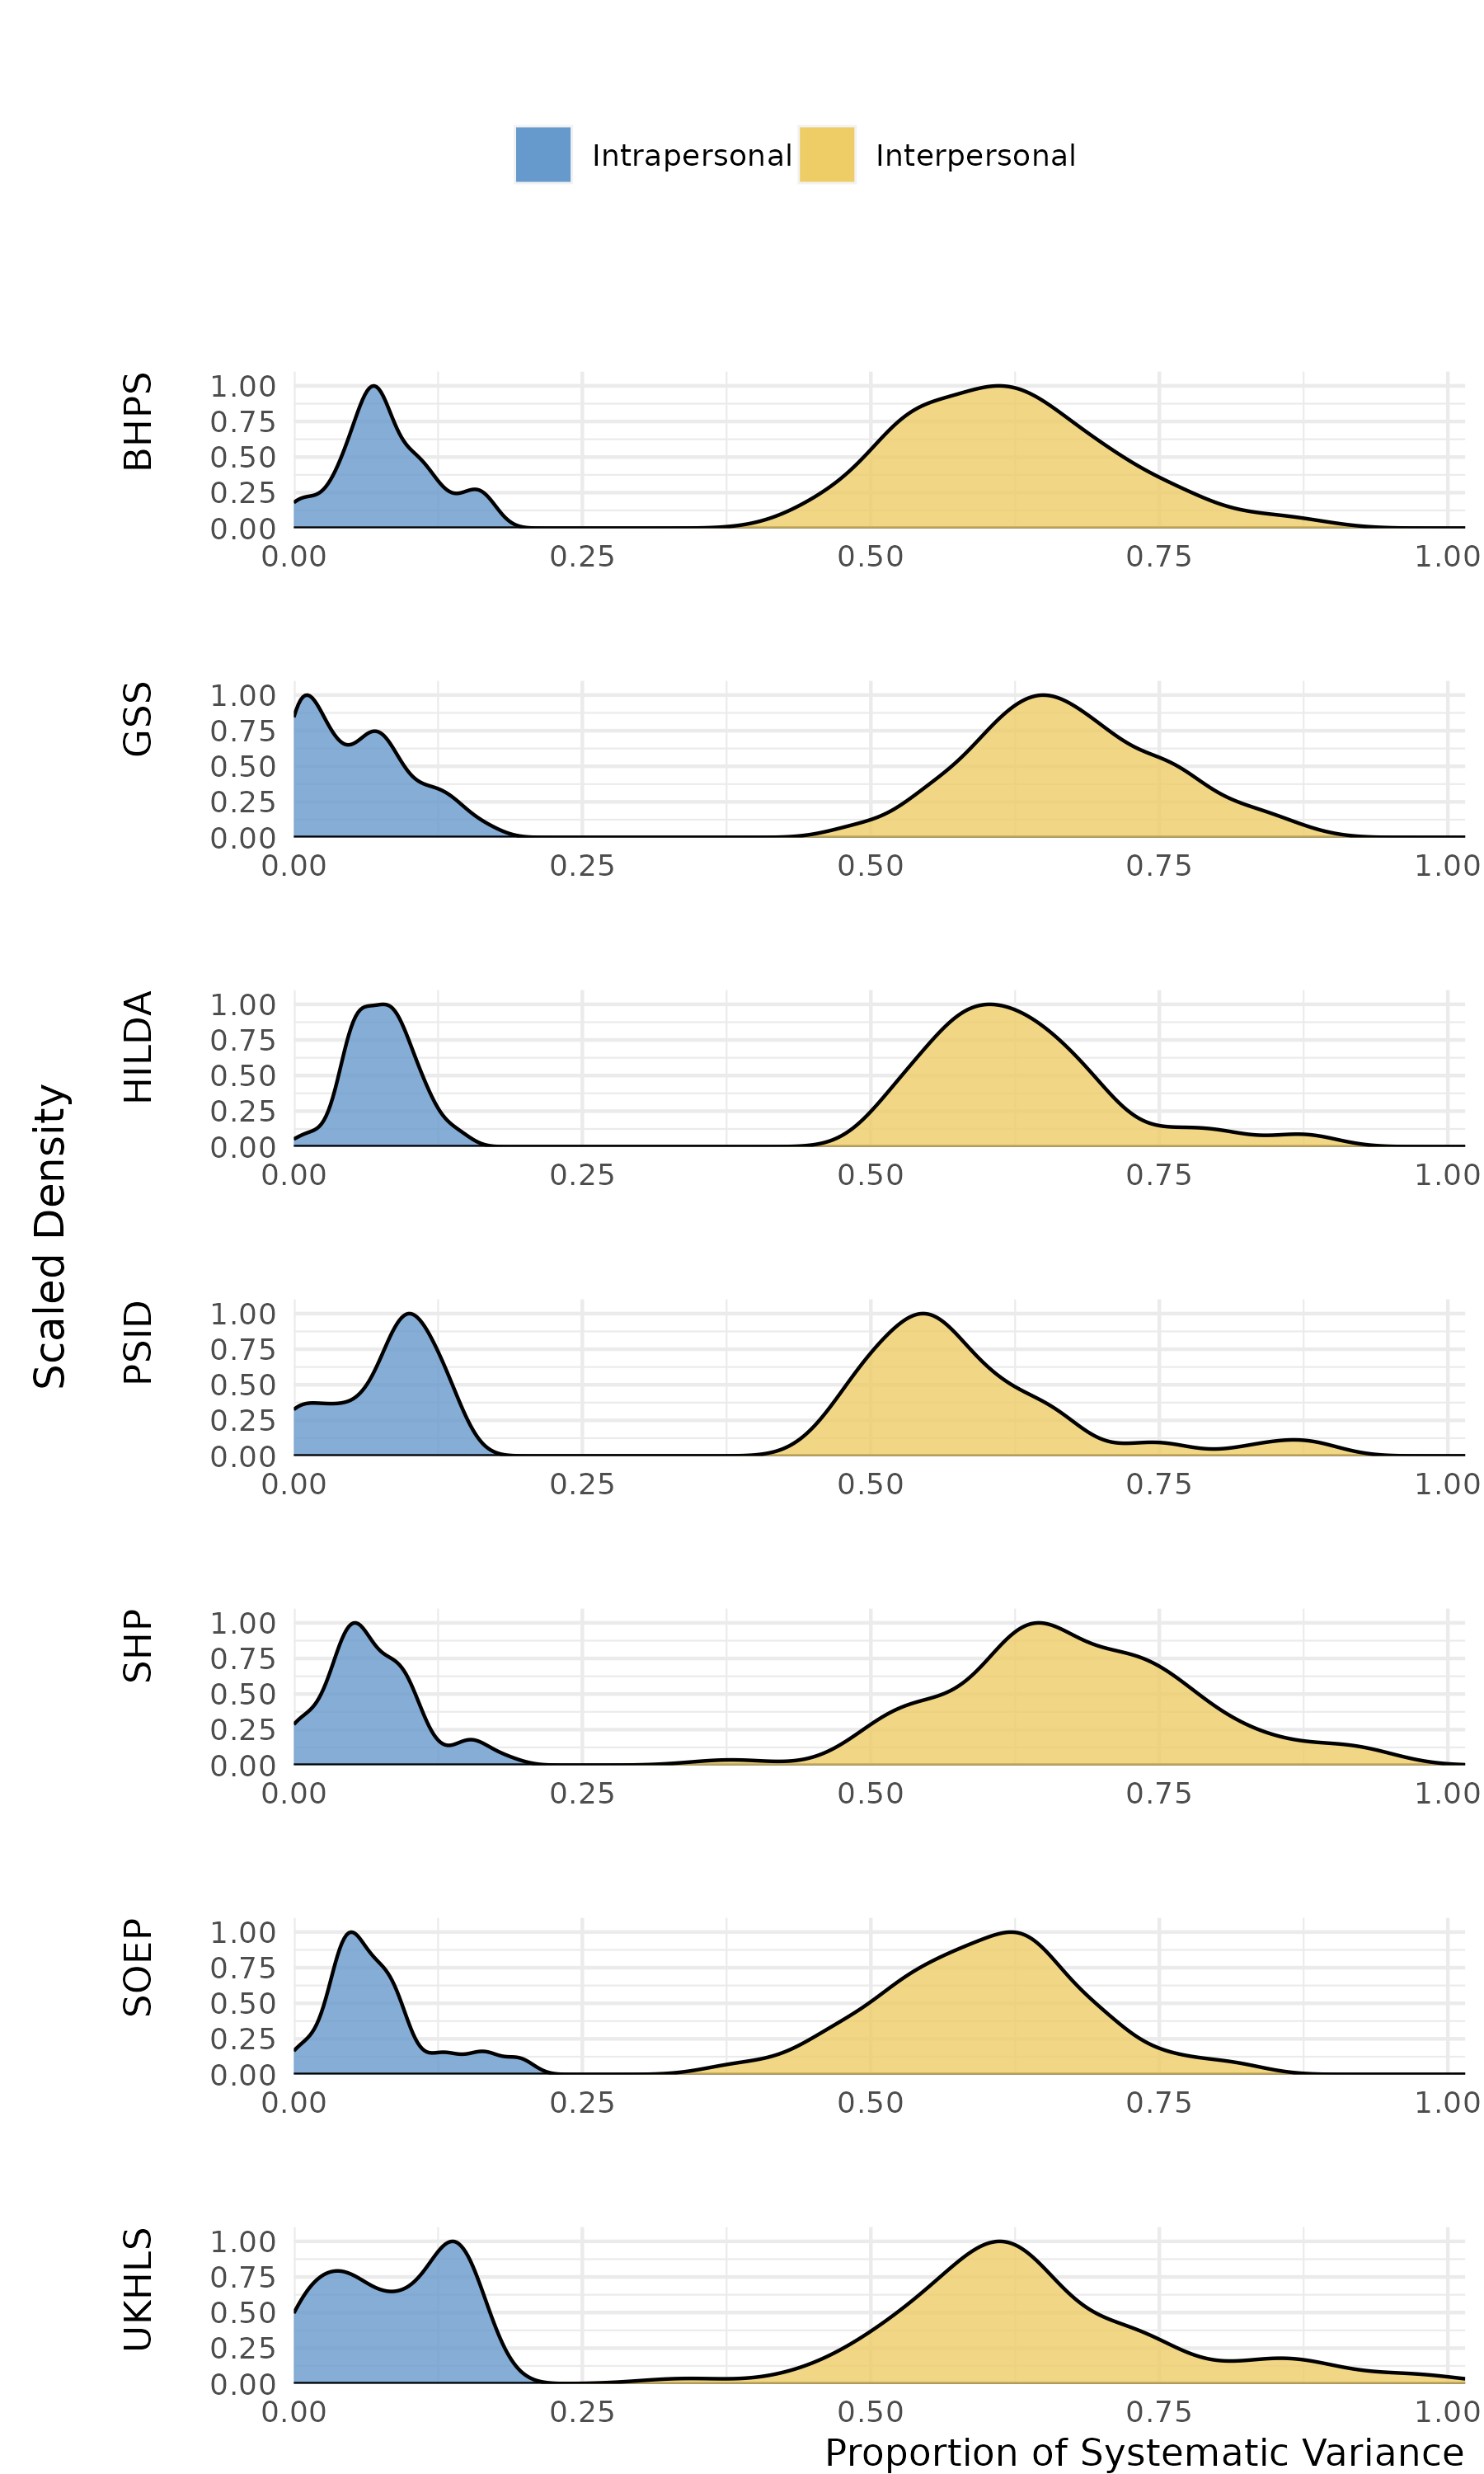
\includegraphics[width=350px]{../figures/figure_A1}

\end{center}
\end{figure}

\hypertarget{appendix-b-omega-values-when-the-last-wave-removed}{%
\subsection{\texorpdfstring{Appendix B: \(\omega\) Values When the Last
Wave
Removed}{Appendix B: \textbackslash omega Values When the Last Wave Removed}}\label{appendix-b-omega-values-when-the-last-wave-removed}}

Figure A2 presents the alternative strategy we used to understand the
effects of duration on intraindividual change. First, we removed the
last wave from all the observations and fitted the Life Course Adaption
models. This effectively reduced the number of items to 249. We then
refitted the model for all participants in this sample using the
unrestricted data. In the final step, we calculated the \(\omega\)
values for each item. The Figure A2 shows a scatterplot for these two
sets of observations.

\begin{figure}[tb]
\begin{center}
\caption*{Figure A2: Difference in $\omega$ Across Two Sample Specifications} 

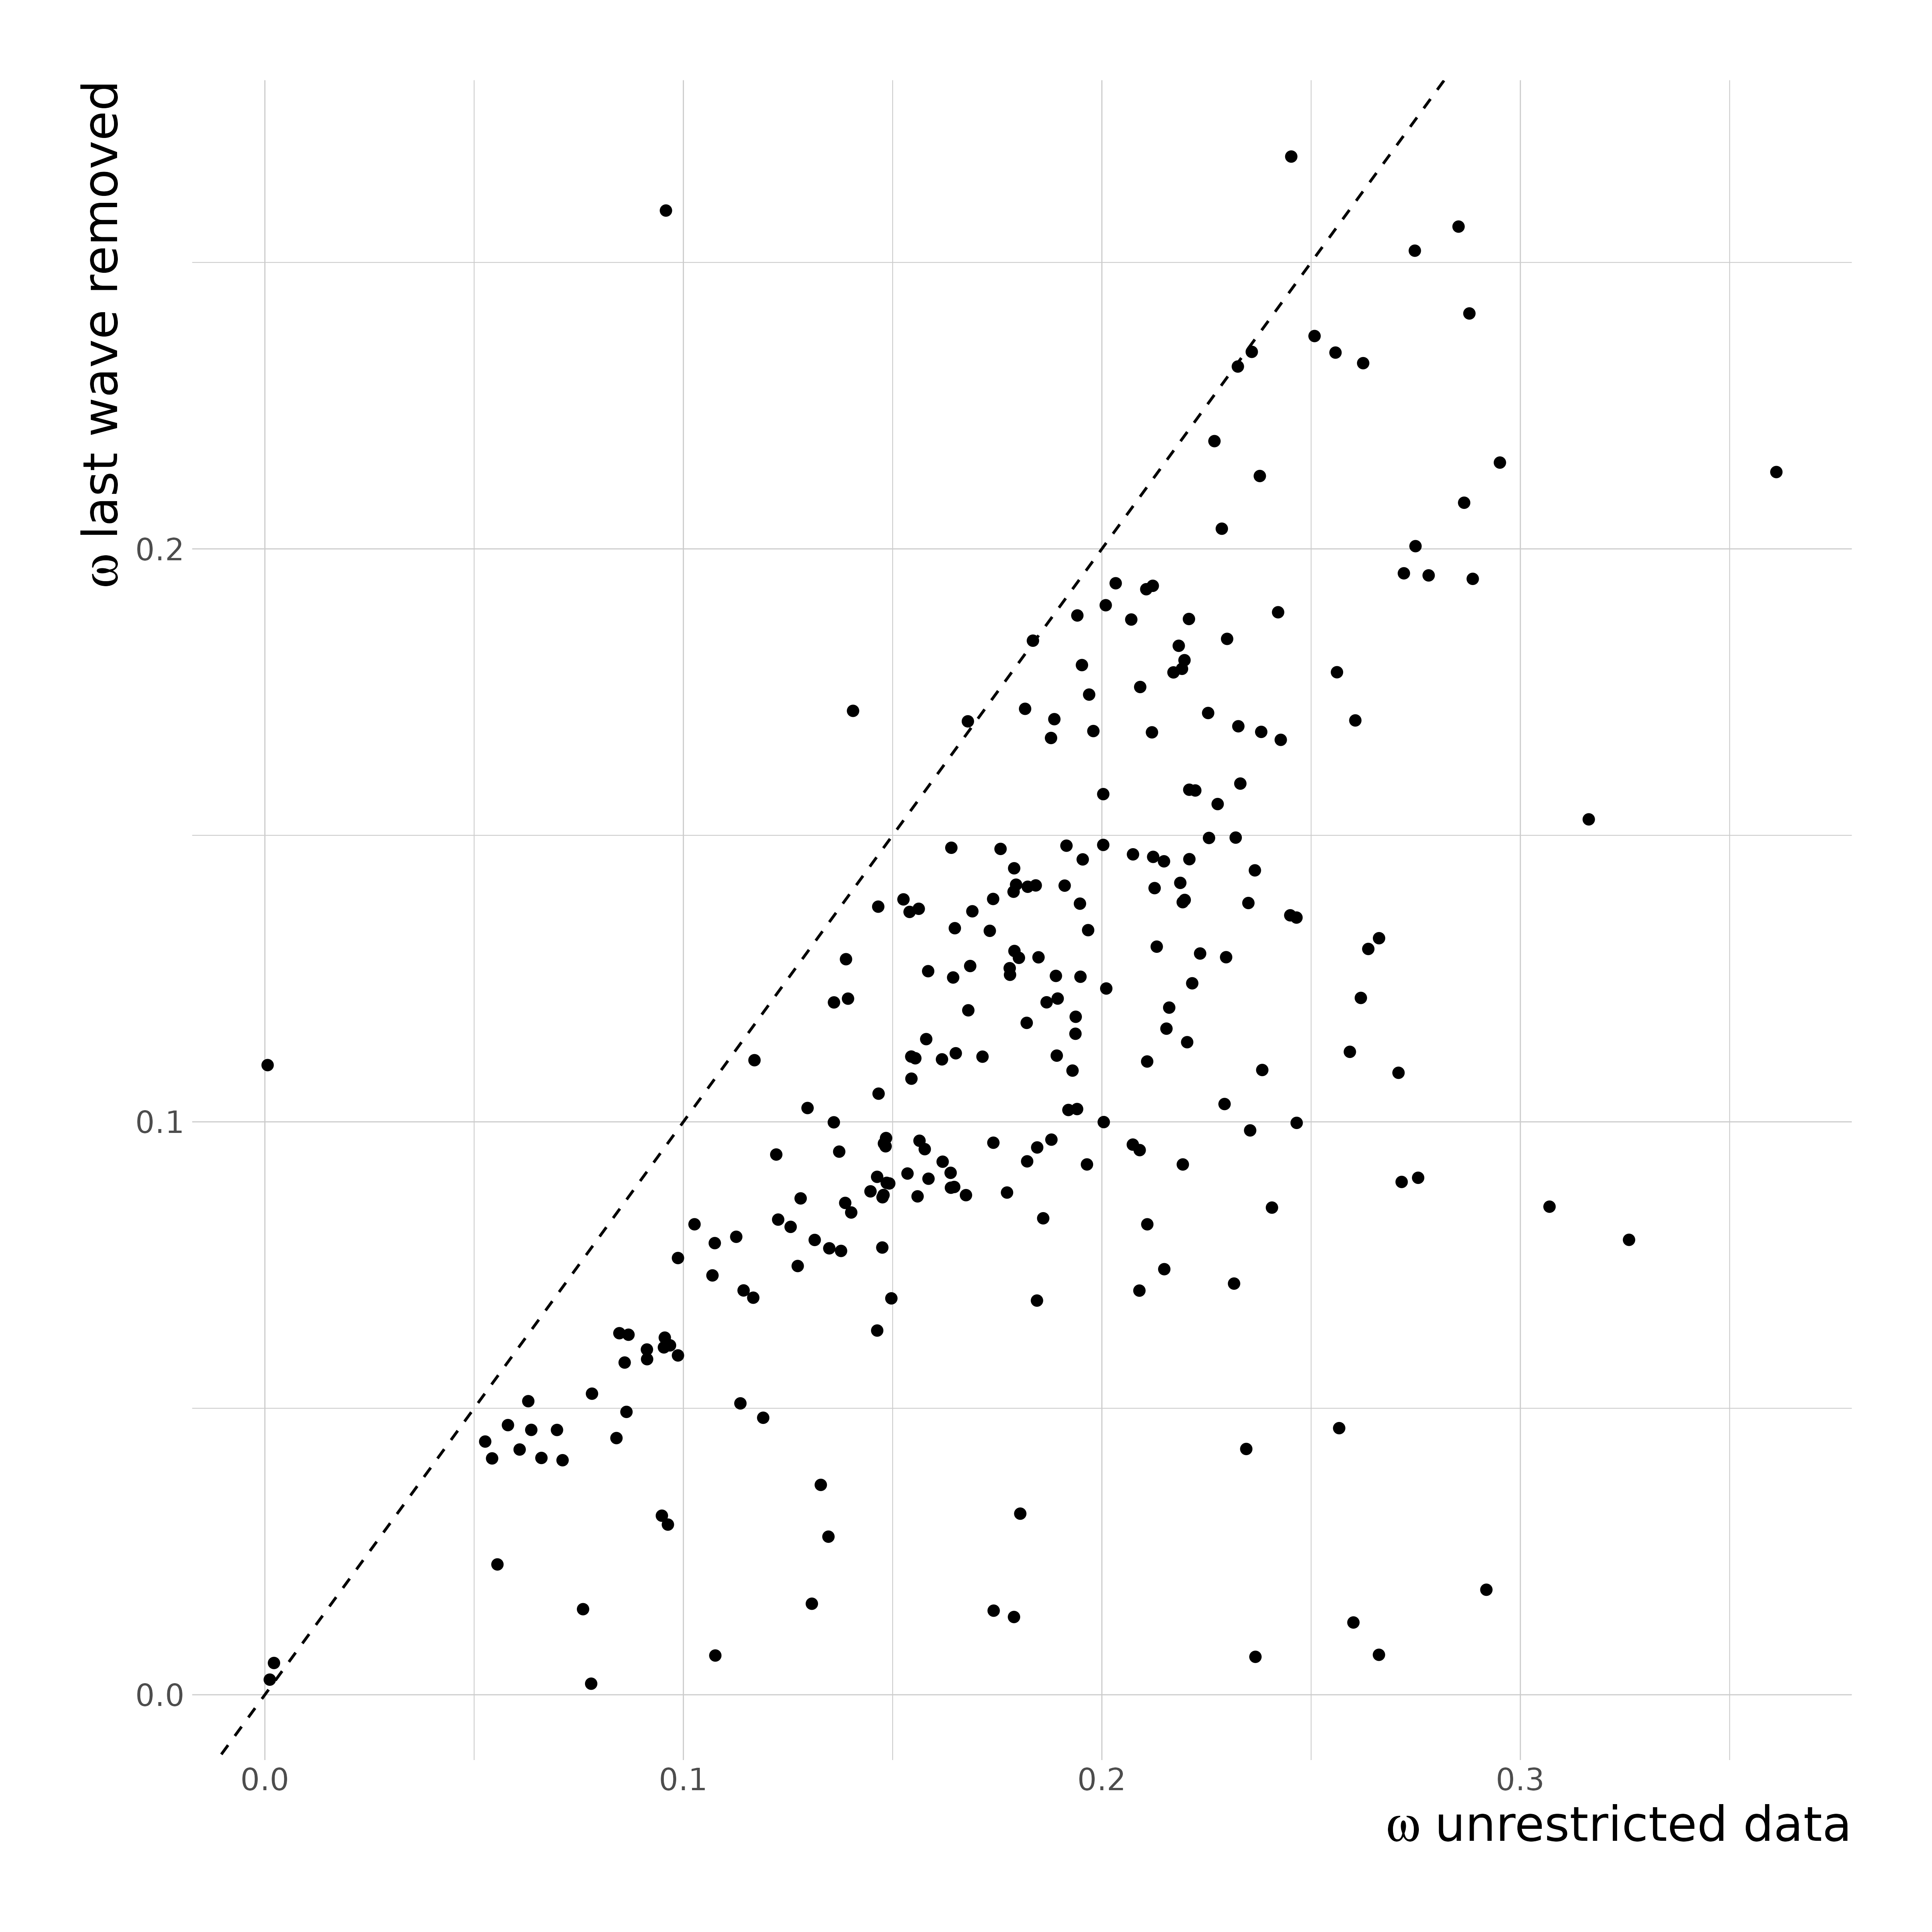
\includegraphics[width=400px]{../figures/figure_A2}

\end{center}
\end{figure}

\end{document}
